\begingroup
\graphicspath{{../prob_2/Figures/}}

% =====================================================
% Problem 2 : Conditional GAN for MNIST Data Generation
% =====================================================

\subsection{Conditional Generative Adversarial Network (GAN)}

In this experiment, a Conditional Generative Adversarial Network (CGAN) was implemented to generate synthetic MNIST handwritten digit images using a limited dataset containing only 350 real samples per digit.

The main objective was to investigate whether GAN-generated synthetic data can improve classifier performance and reduce the dependence on large real datasets.

In addition, the experiment compares GAN-generated data against traditional augmentation techniques used in Assignment 2.

% =====================================================
\subsubsection{Pipeline Overview}

The implemented GAN pipeline is summarized as follows:

\begin{enumerate}

    \item Load and preprocess the MNIST dataset.
    
    \item Reduce the dataset to 350 real samples per digit.
    
    \item Apply augmentation using:
    
    \begin{itemize}
        \item Rotation
        \item Translation
        \item Scaling
        \item Gaussian noise
    \end{itemize}
    
    \item Train a Conditional GAN using the augmented dataset.
    
    \item Repeat GAN training for 5 independent runs using different random initialization.
    
    \item Generate synthetic digit samples from each GAN model.
    
    \item Train a LeNet-5 classifier using the reduced real dataset.
    
    \item Classify generated images and compute:
    
    \[
    \text{confidence} = \max(\text{softmax output})
    \]
    
    \item Construct three synthetic datasets:
    
    \begin{itemize}
        \item Set A: all generated samples
        \item Set B: confidence $\geq 0.9$
        \item Set C: $0.6 \leq \text{confidence} < 0.9$
    \end{itemize}
    
    \item Retrain LeNet-5 using:
    
    \begin{itemize}
        \item 350 real samples only
        \item 350 real + Set A
        \item 350 real + Set B
        \item 350 real + Set C
    \end{itemize}
    
    \item Compare against:
    
    \begin{itemize}
        \item 350-real baseline
        \item 1000-real baseline
        \item Augmentation-only results from Assignment 2
    \end{itemize}

\end{enumerate}

% =====================================================
\subsubsection{Pipeline Flowchart}

\definecolor{softblue}{RGB}{173,216,230}
\definecolor{softgreen}{RGB}{190,230,200}
\definecolor{softpurple}{RGB}{220,210,255}
\definecolor{softorange}{RGB}{255,220,180}
\definecolor{softred}{RGB}{255,200,200}

\begin{figure}[H]
\centering

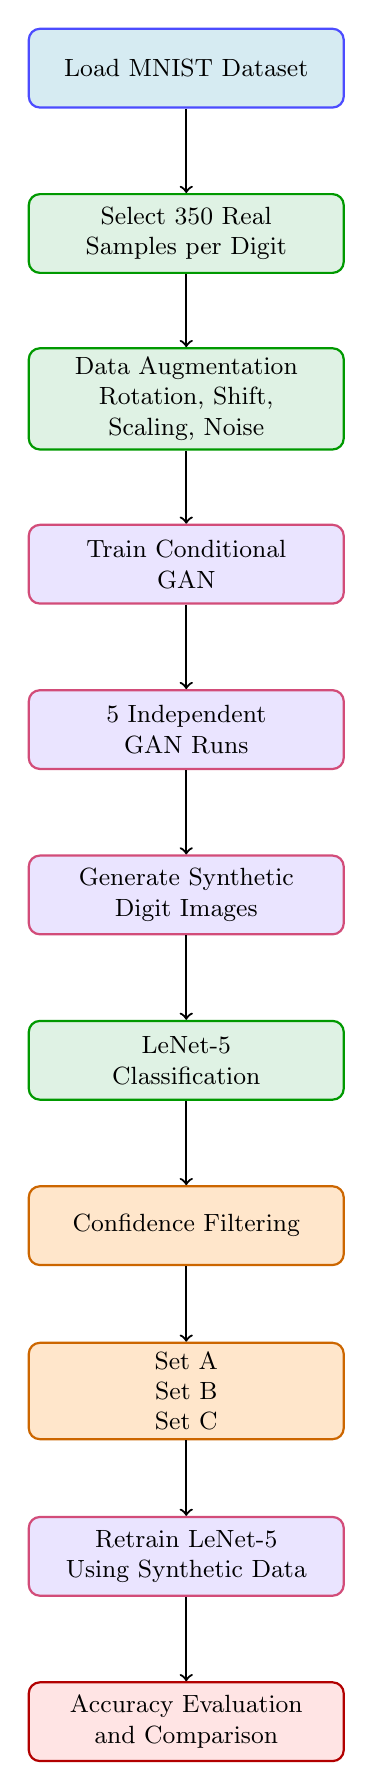
\begin{tikzpicture}[
node distance=2.1cm,
every node/.style={
align=center,
minimum width=4cm,
minimum height=1cm,
font=\small
},
arrow/.style={->, thick}
]

% =====================================================
% Styles
% =====================================================

\tikzstyle{input} =
[rectangle, rounded corners,
fill=softblue!50,
draw=blue!70,
thick]

\tikzstyle{process} =
[rectangle, rounded corners,
fill=softgreen!50,
draw=green!60!black,
thick]

\tikzstyle{model} =
[rectangle, rounded corners,
fill=softpurple!60,
draw=purple!70,
thick]

\tikzstyle{filter} =
[rectangle, rounded corners,
fill=softorange!70,
draw=orange!80!black,
thick]

\tikzstyle{output} =
[rectangle, rounded corners,
fill=softred!50,
draw=red!70!black,
thick]

% =====================================================
% Nodes
% =====================================================

\node (mnist) [input]
{Load MNIST Dataset};

\node (reduce) [process, below of=mnist]
{Select 350 Real\\Samples per Digit};

\node (augment) [process, below of=reduce]
{Data Augmentation\\Rotation, Shift,\\Scaling, Noise};

\node (traingan) [model, below of=augment]
{Train Conditional\\GAN};

\node (runs) [model, below of=traingan]
{5 Independent\\GAN Runs};

\node (generate) [model, below of=runs]
{Generate Synthetic\\Digit Images};

\node (classifier) [process, below of=generate]
{LeNet-5\\Classification};

\node (confidence) [filter, below of=classifier]
{Confidence Filtering};

\node (sets) [filter, below of=confidence]
{Set A\\Set B\\Set C};

\node (retrain) [model, below of=sets]
{Retrain LeNet-5\\Using Synthetic Data};

\node (evaluate) [output, below of=retrain]
{Accuracy Evaluation\\and Comparison};

% =====================================================
% Arrows
% =====================================================

\draw [arrow] (mnist) -- (reduce);

\draw [arrow] (reduce) -- (augment);

\draw [arrow] (augment) -- (traingan);

\draw [arrow] (traingan) -- (runs);

\draw [arrow] (runs) -- (generate);

\draw [arrow] (generate) -- (classifier);

\draw [arrow] (classifier) -- (confidence);

\draw [arrow] (confidence) -- (sets);

\draw [arrow] (sets) -- (retrain);

\draw [arrow] (retrain) -- (evaluate);

\end{tikzpicture}

\caption{Conditional GAN synthetic data generation pipeline.}

\label{fig:gan_pipeline}

\end{figure}

% =====================================================
\subsubsection{Augmented Training Samples}

Figure~\ref{fig:gan_aug} shows examples of augmented MNIST samples used during GAN training.

\begin{figure}[H]
\centering
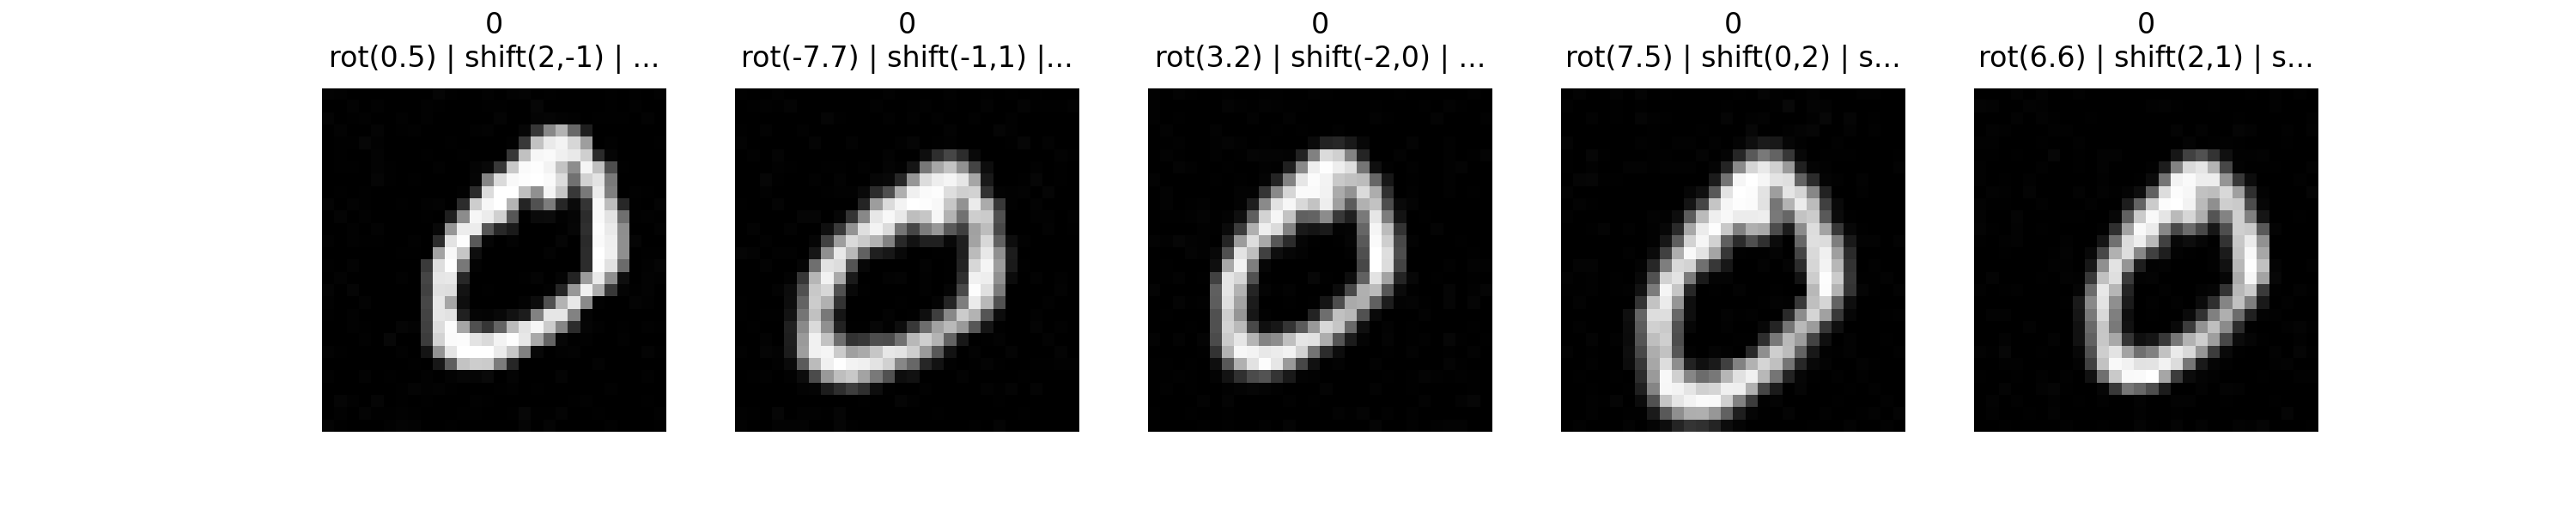
\includegraphics[width=\linewidth]{GAN_aug_samples.png}
\caption{Augmented MNIST samples used for GAN training.}
\label{fig:gan_aug}
\end{figure}

% =====================================================
\subsubsection{GAN Architecture}

The implemented Conditional GAN consists of:

\begin{itemize}

    \item \textbf{Generator}
    
    \begin{itemize}
        \item Latent noise input
        \item Label embedding
        \item Dense projection
        \item Transposed convolution layers
        \item Tanh output activation
    \end{itemize}
    
    \item \textbf{Discriminator}
    
    \begin{itemize}
        \item Convolutional feature extraction
        \item Label conditioning
        \item LeakyReLU activations
        \item Binary classification output
    \end{itemize}

\end{itemize}

The GAN was trained using adversarial learning where:

\begin{itemize}
    \item The generator attempts to fool the discriminator.
    \item The discriminator attempts to distinguish real from fake images.
\end{itemize}

% =====================================================
\subsubsection{GAN Training Curves}

Figures~\ref{fig:gan_loss1} -- \ref{fig:gan_loss5} show discriminator and generator losses for the five independent GAN runs.

\begin{figure}[H]
\centering
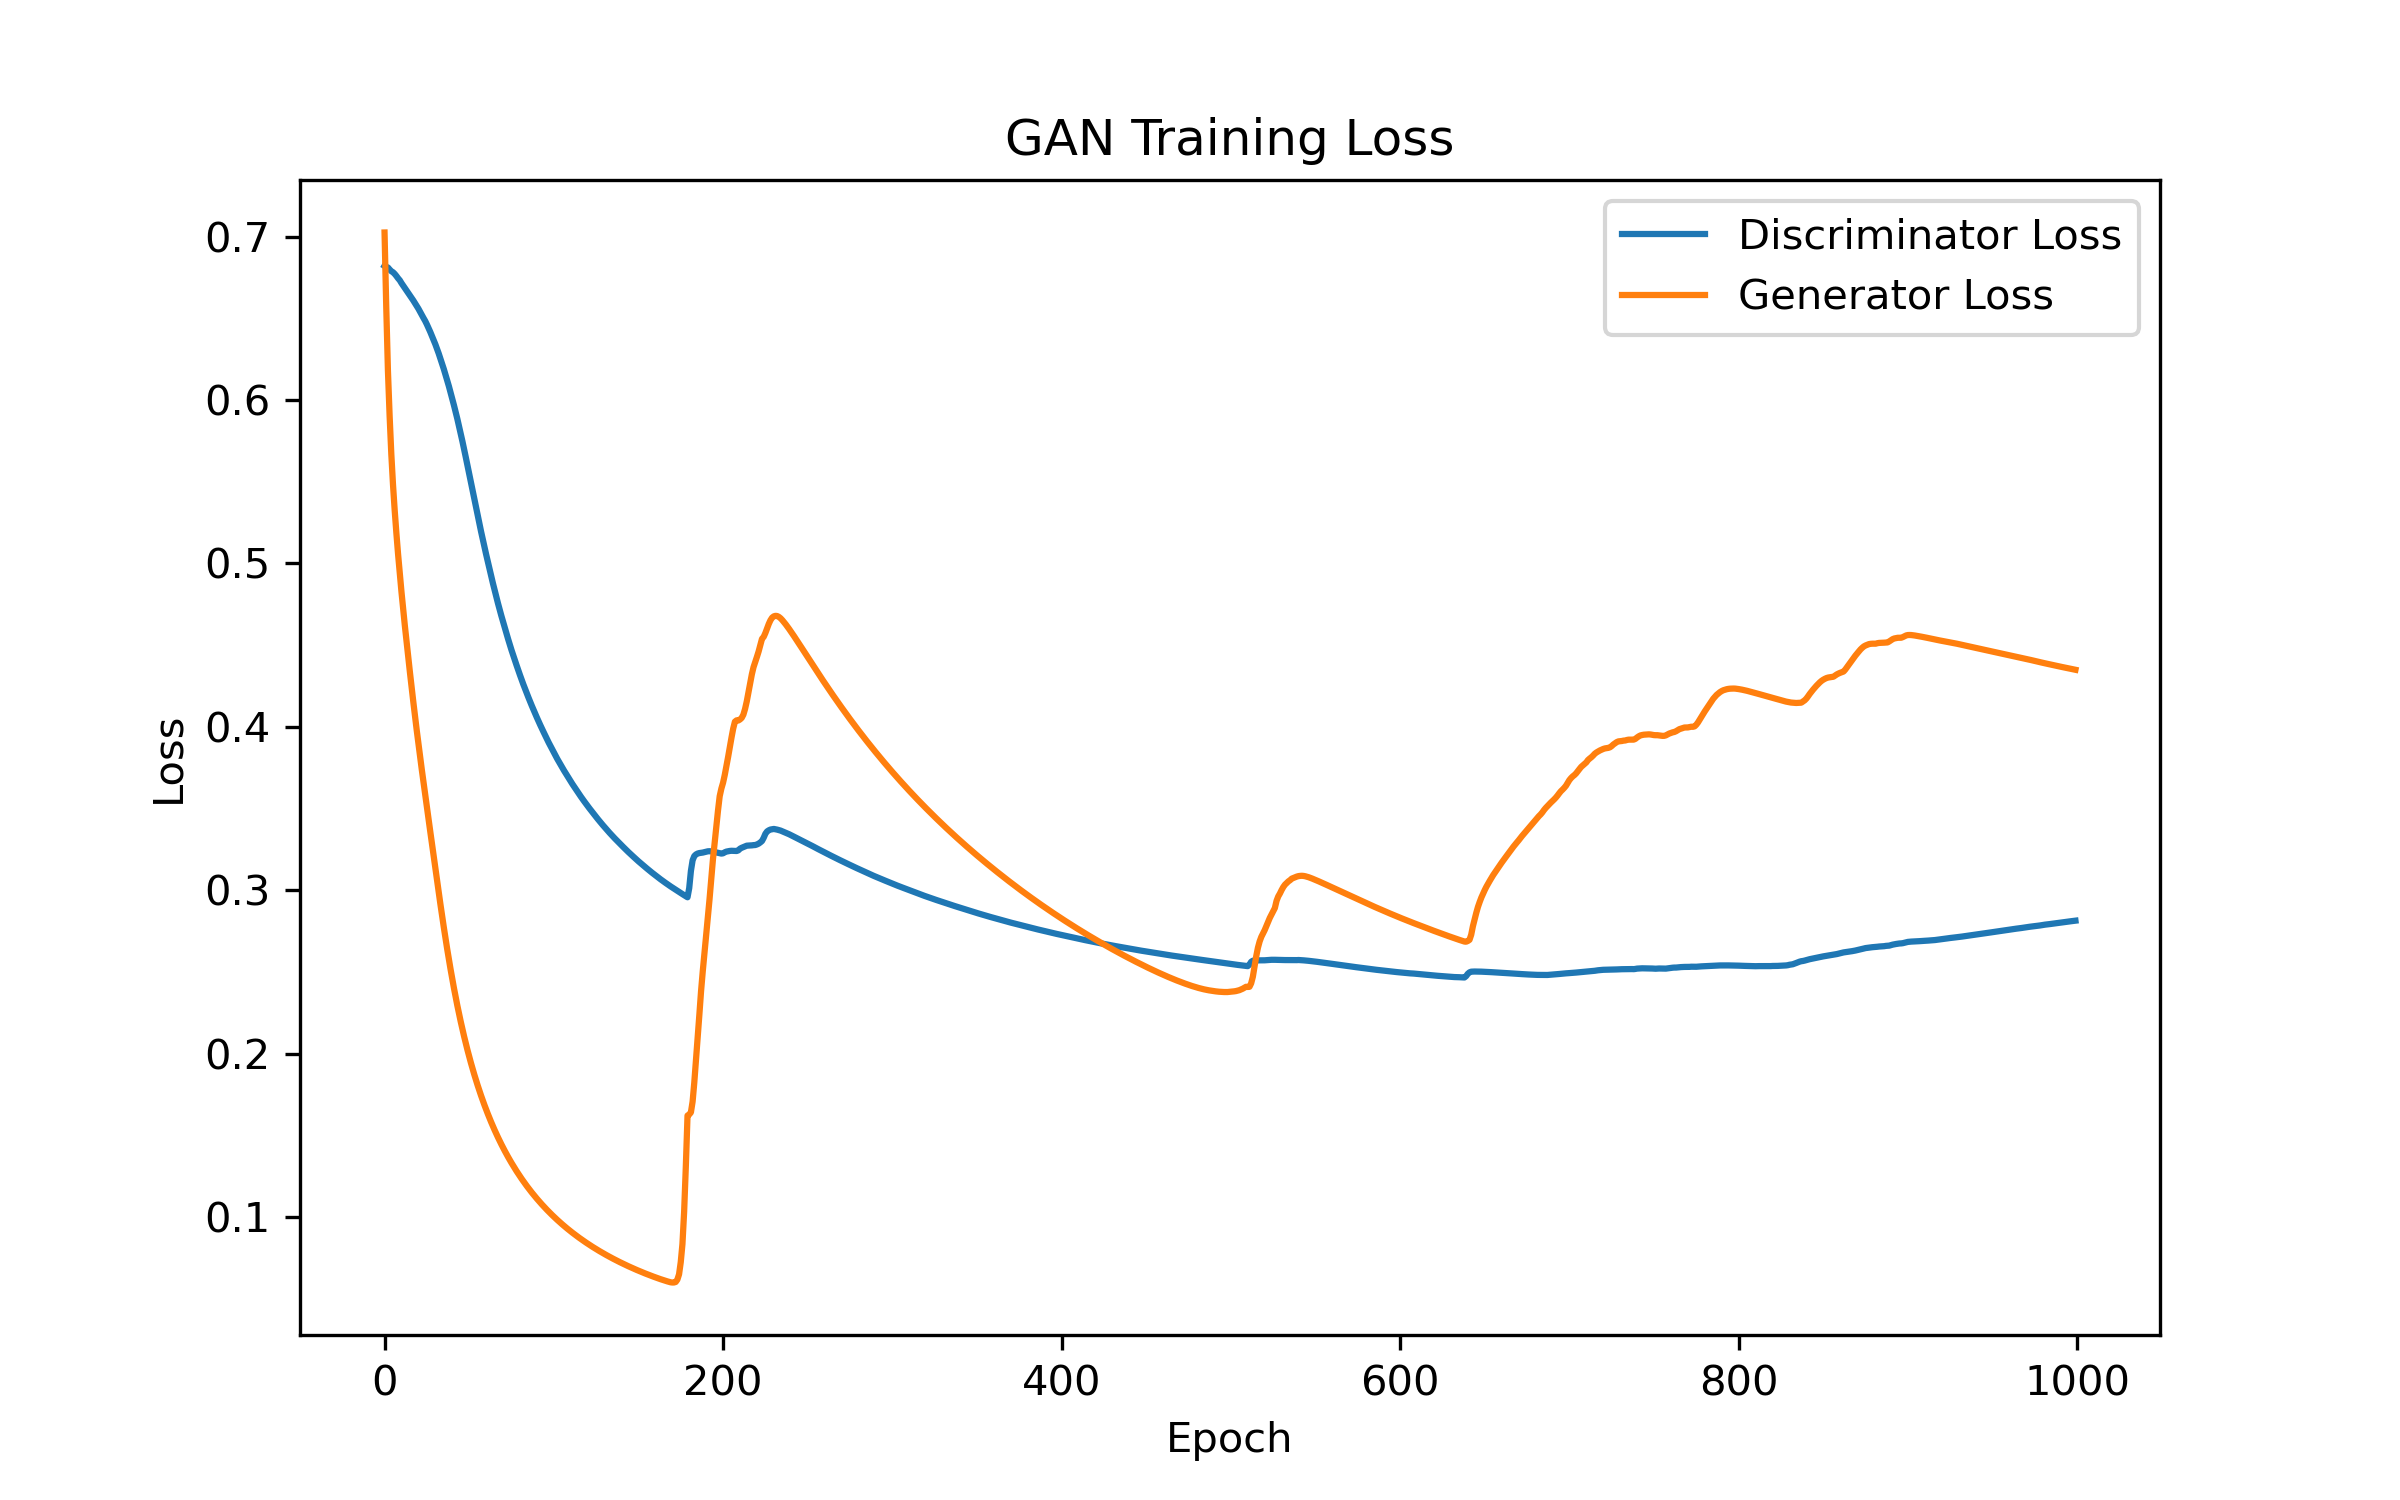
\includegraphics[width=0.9\linewidth]{gan_loss_curve_run_1.png}
\caption{GAN loss curves for Run 1.}
\label{fig:gan_loss1}
\end{figure}

\begin{figure}[H]
\centering
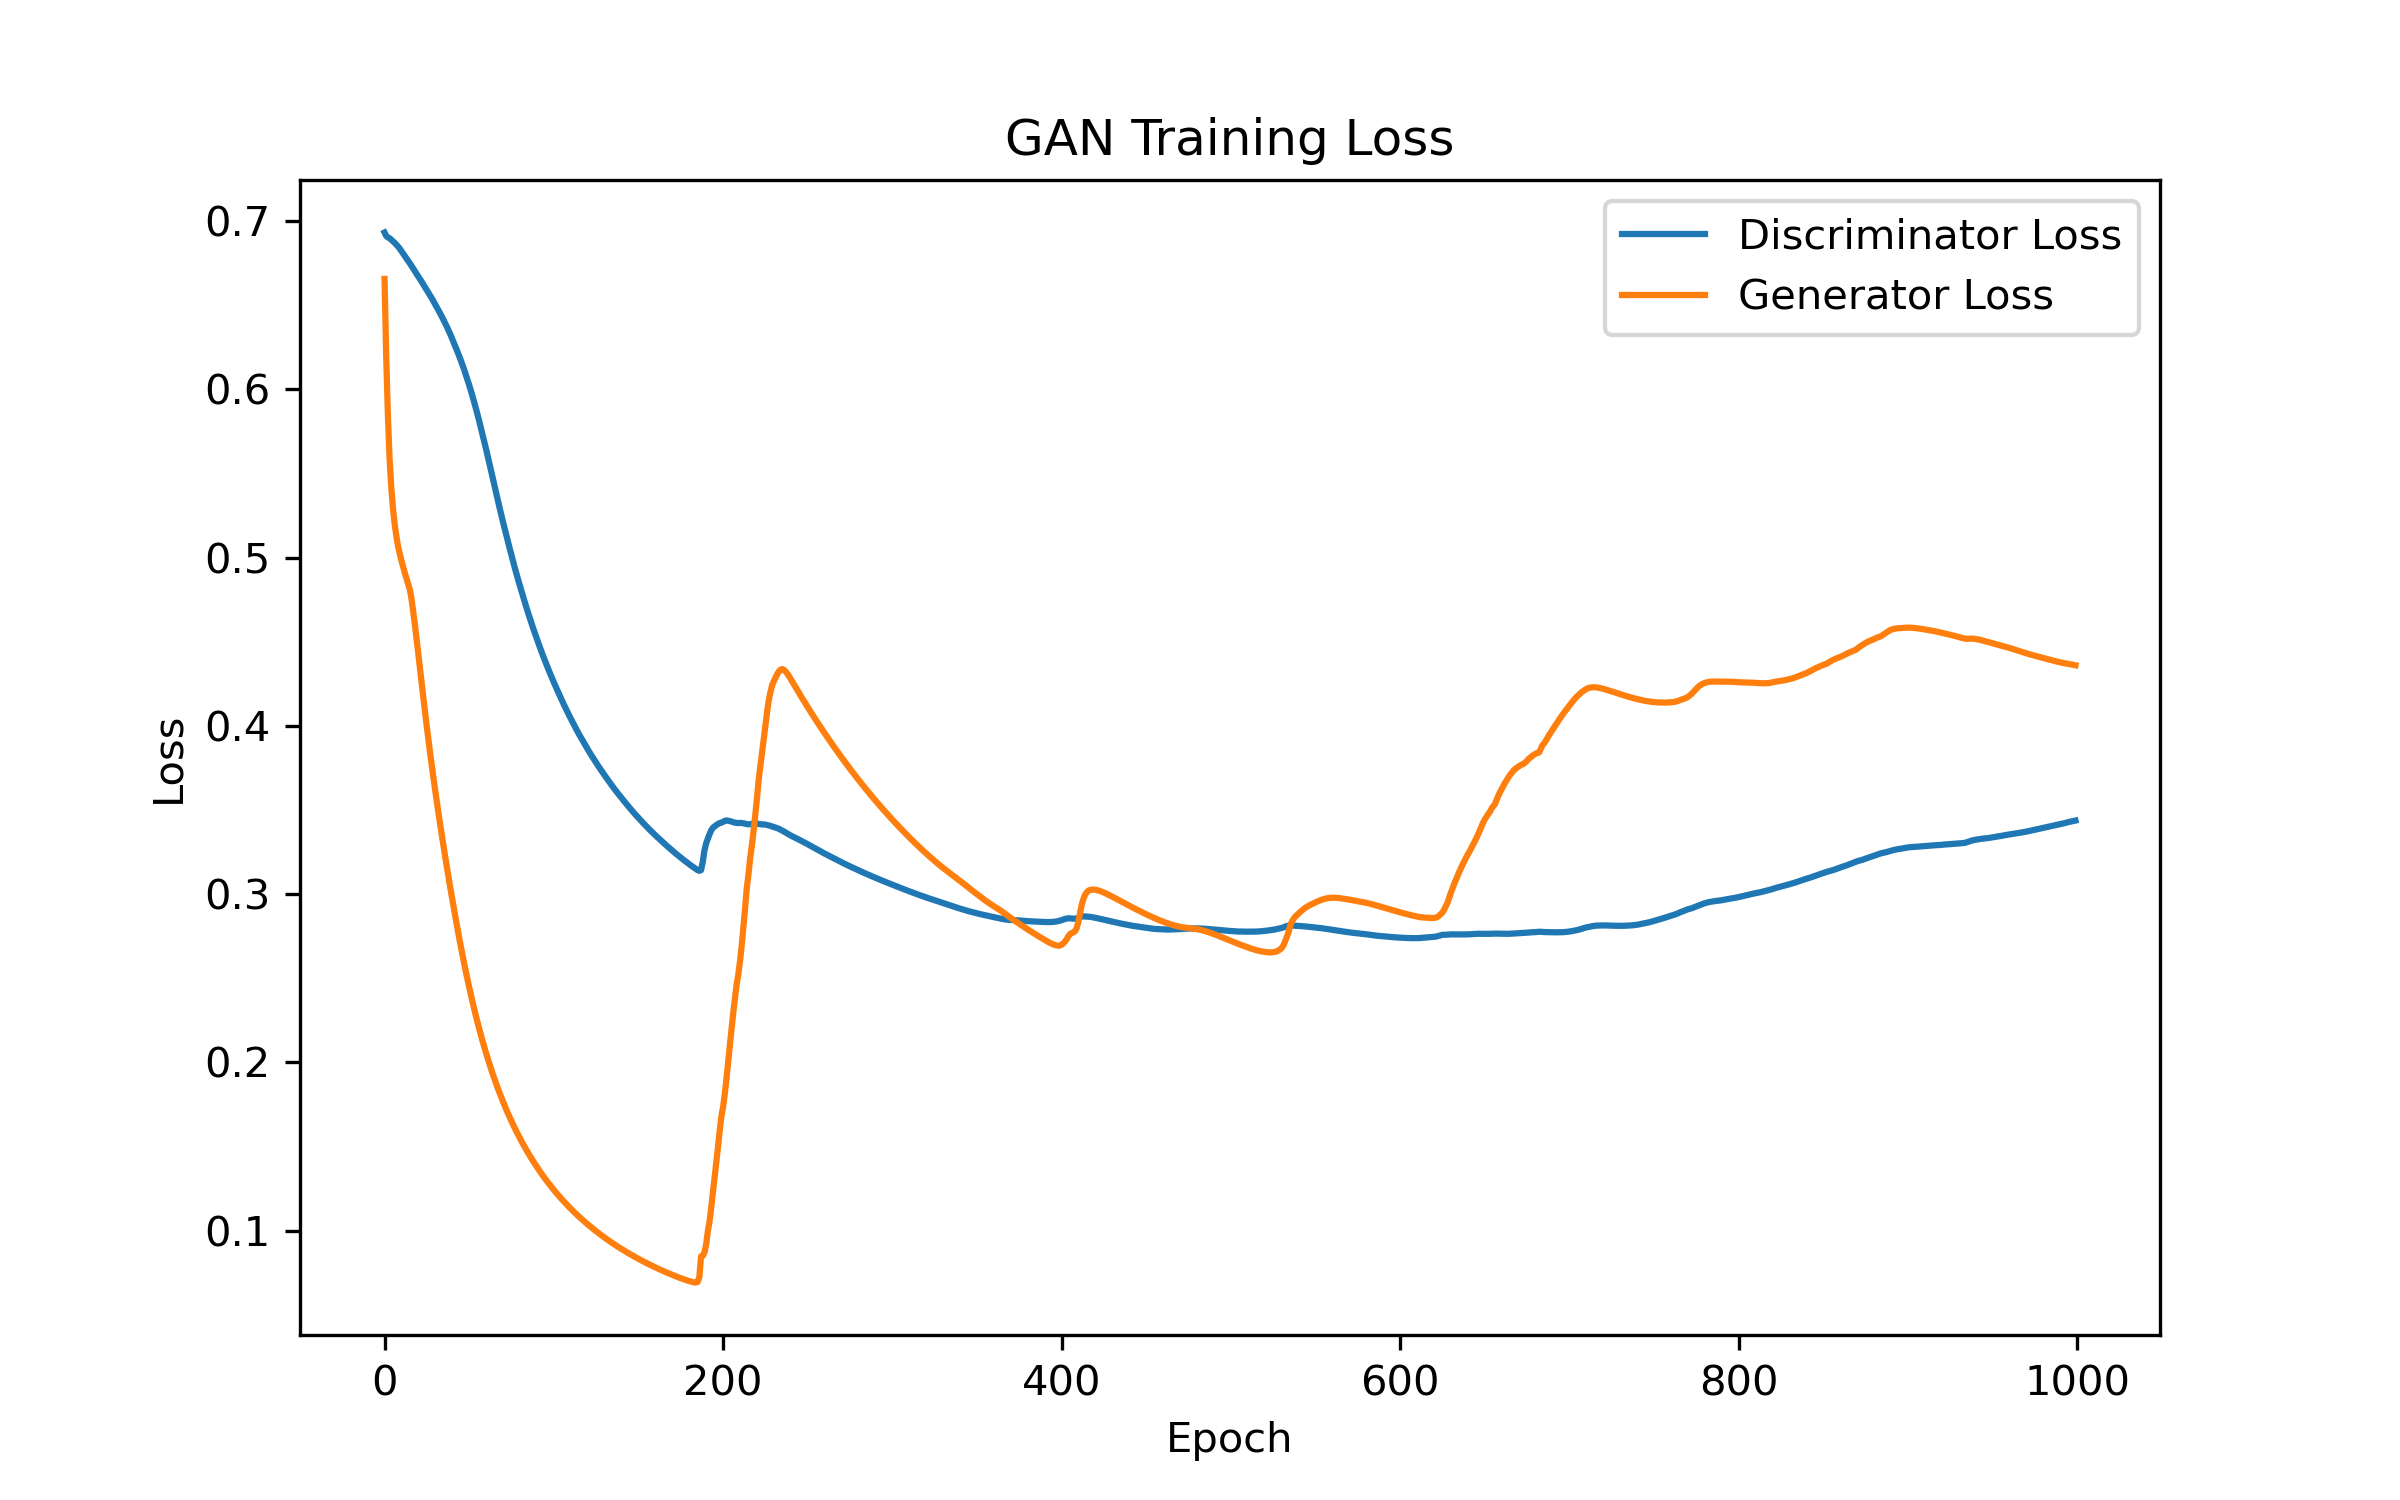
\includegraphics[width=0.9\linewidth]{gan_loss_curve_run_2.png}
\caption{GAN loss curves for Run 2.}
\label{fig:gan_loss2}
\end{figure}

\begin{figure}[H]
\centering
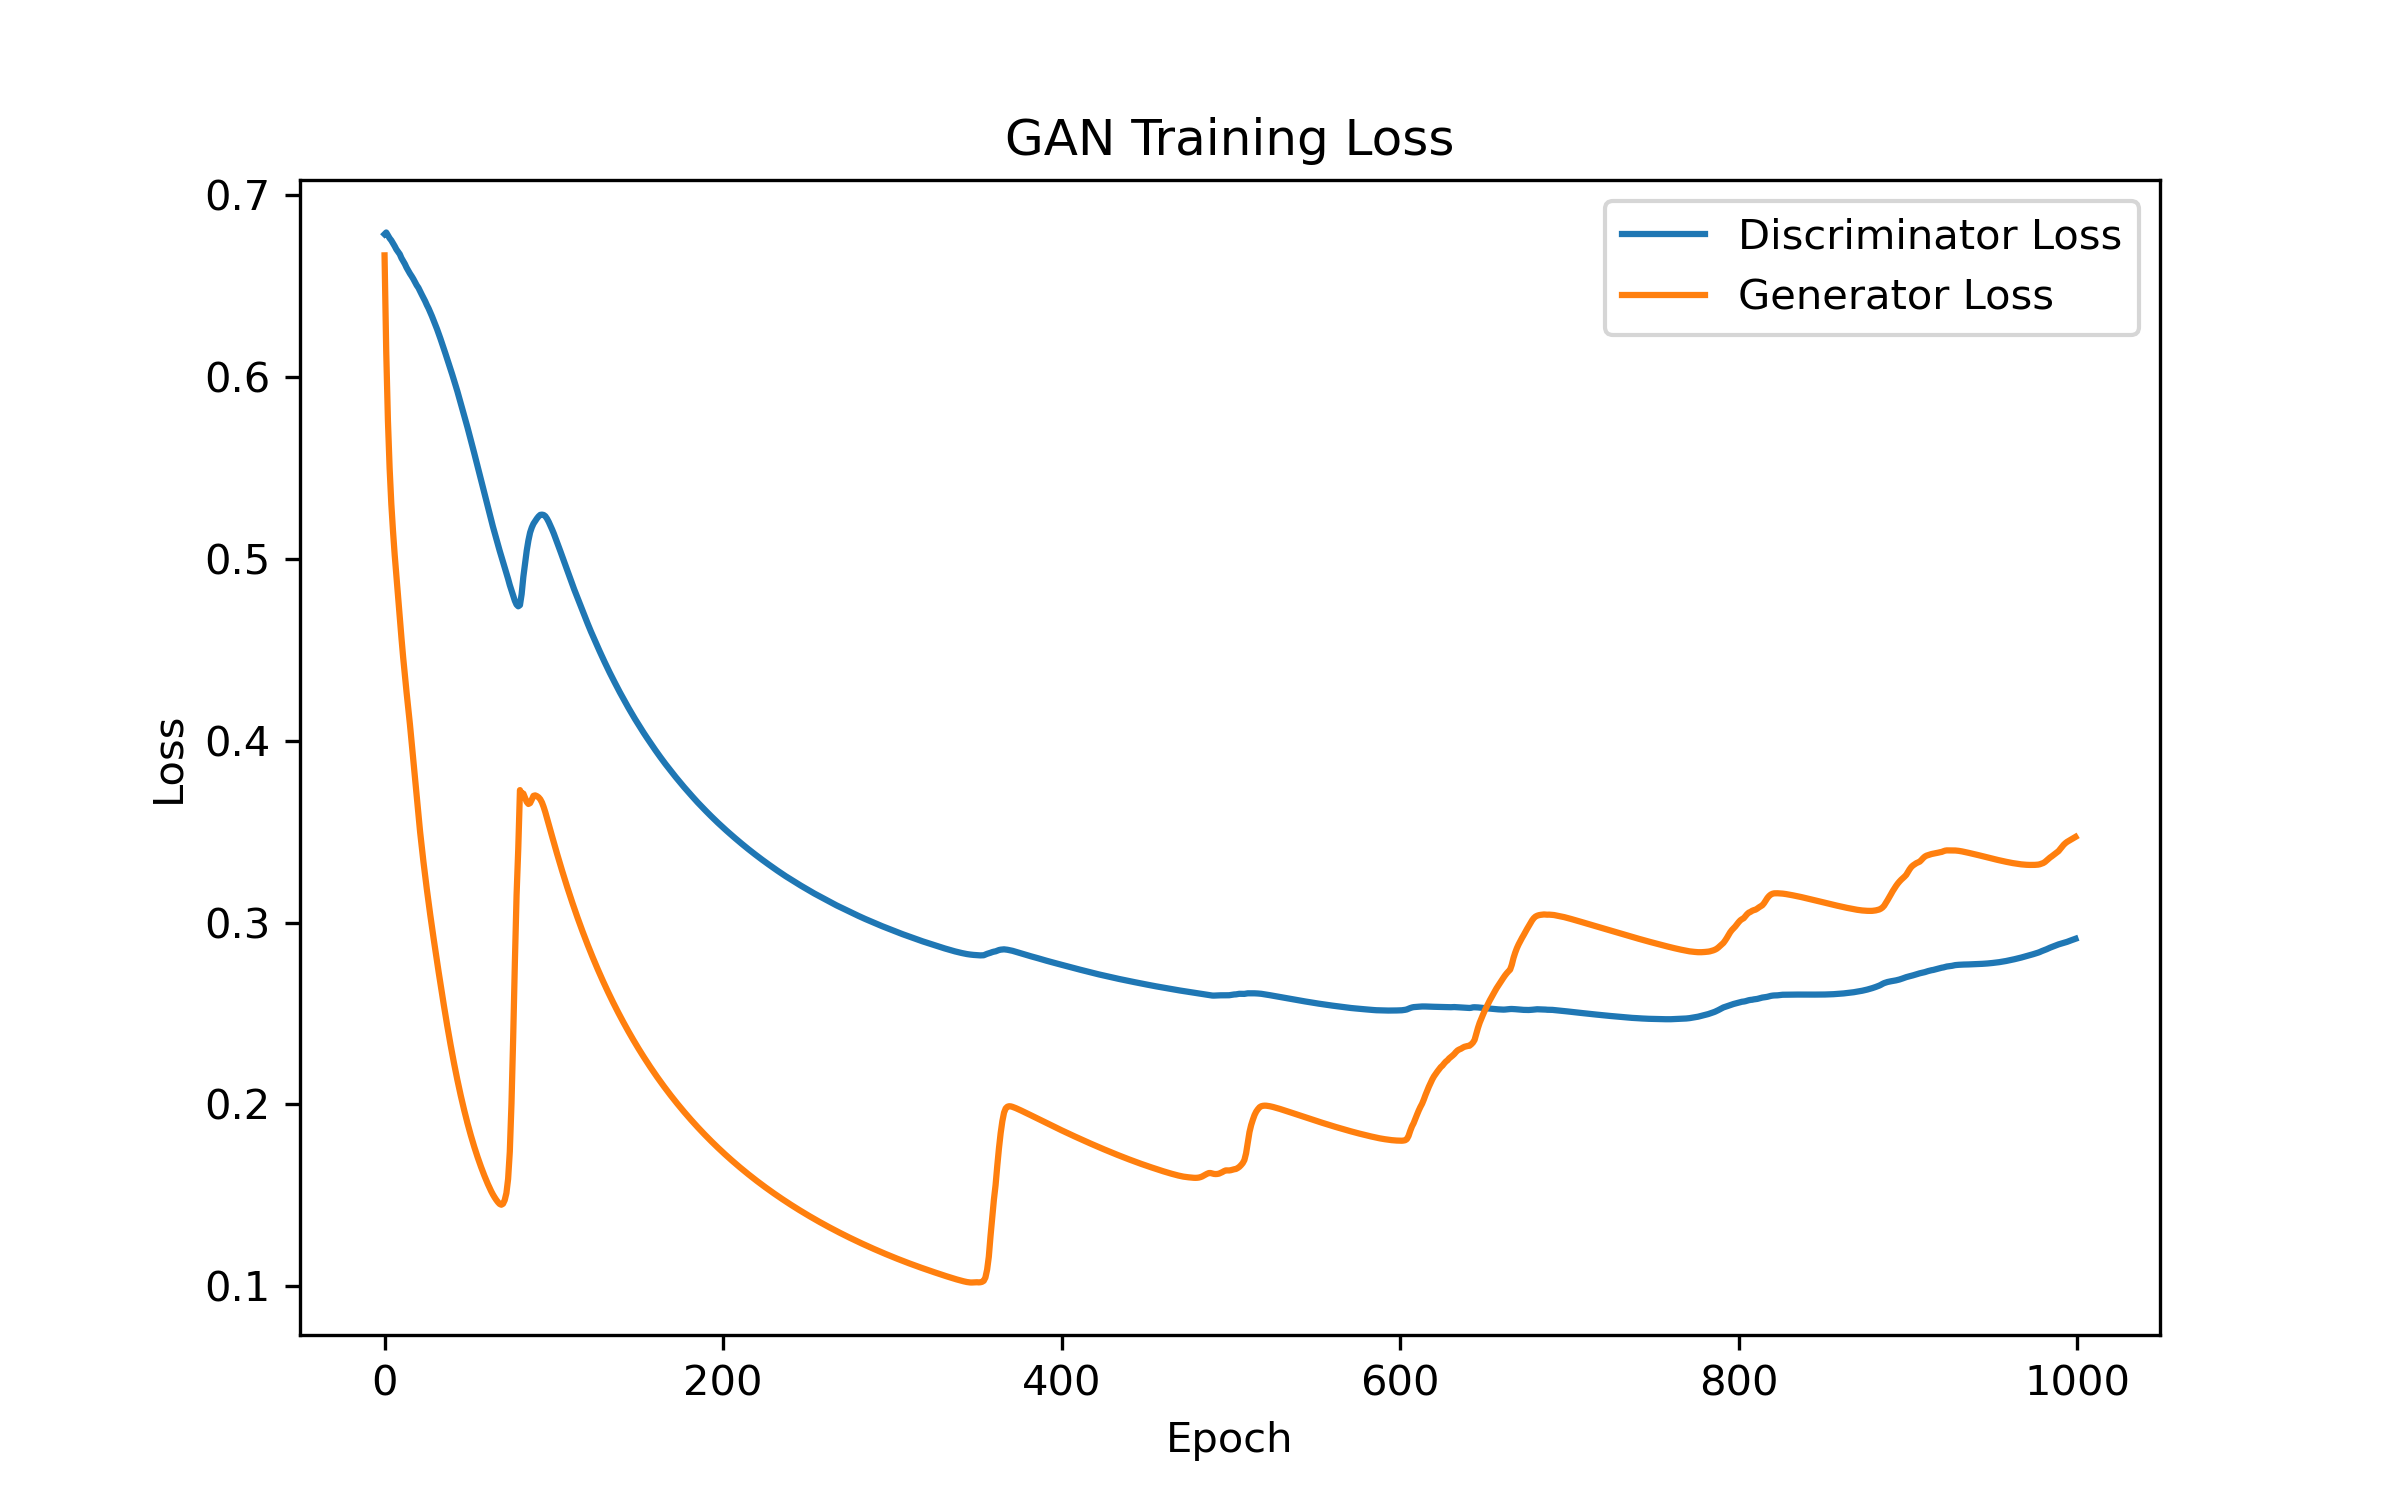
\includegraphics[width=0.9\linewidth]{gan_loss_curve_run_3.png}
\caption{GAN loss curves for Run 3.}
\label{fig:gan_loss3}
\end{figure}

\begin{figure}[H]
\centering
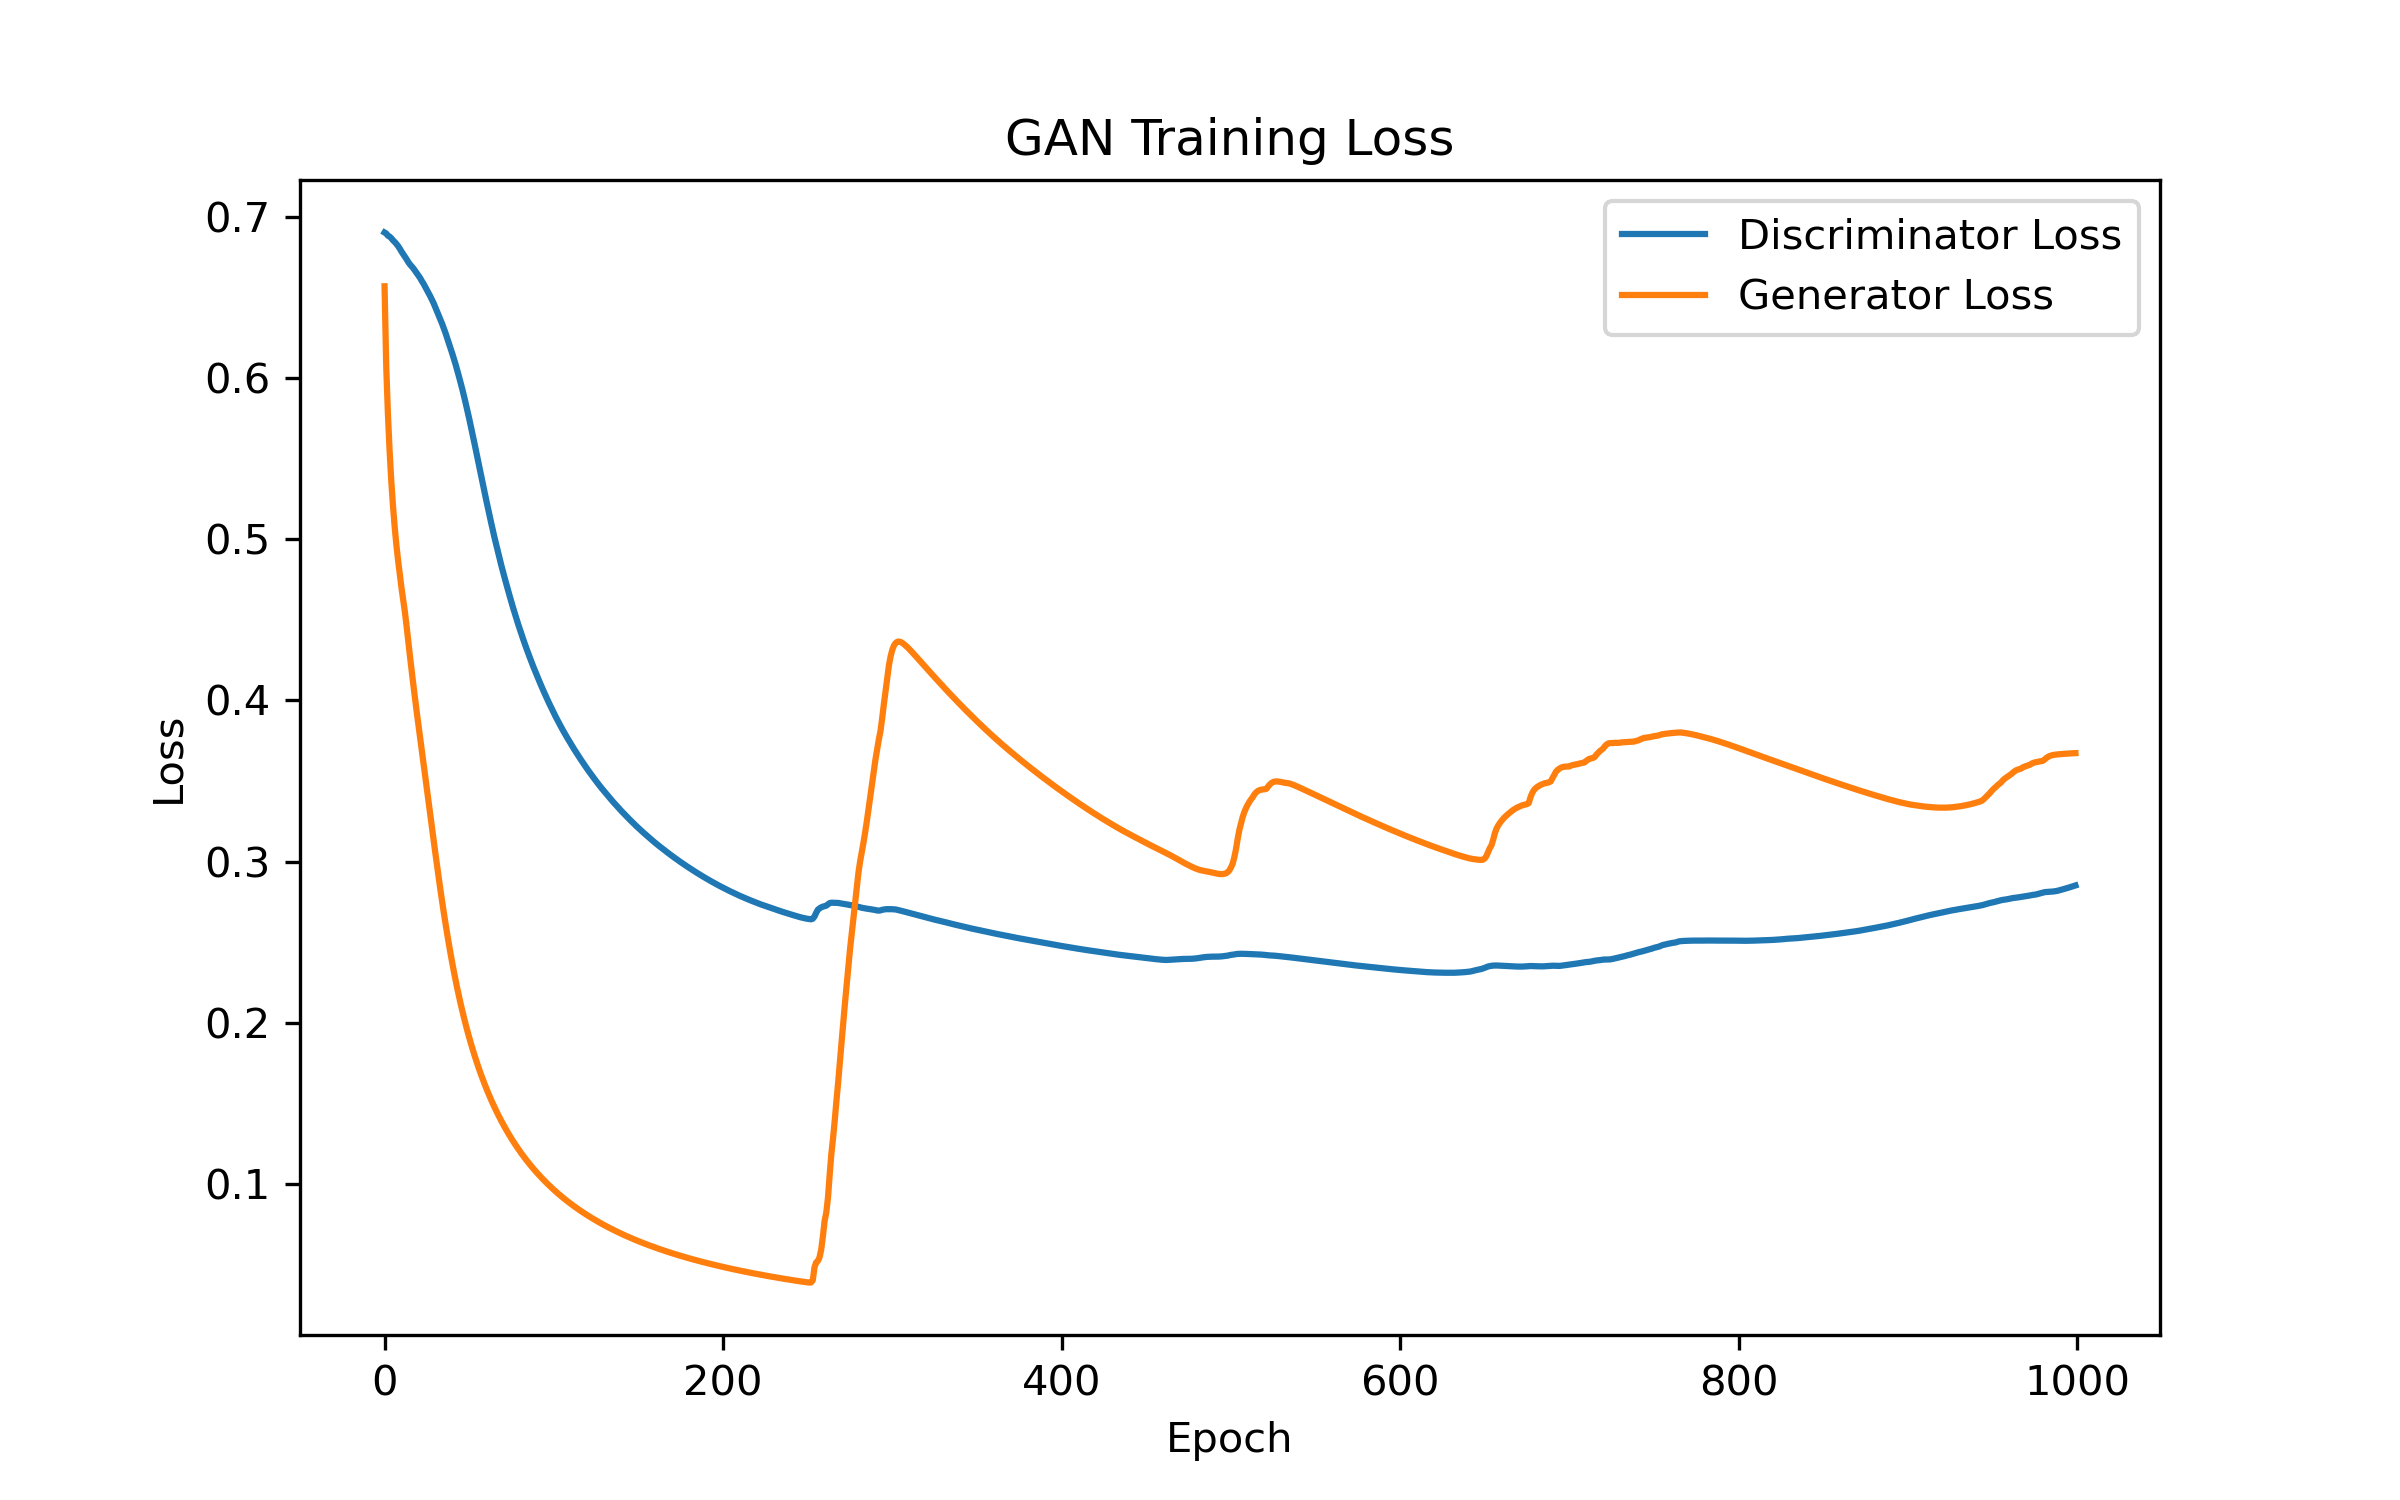
\includegraphics[width=0.9\linewidth]{gan_loss_curve_run_4.png}
\caption{GAN loss curves for Run 4.}
\label{fig:gan_loss4}
\end{figure}

\begin{figure}[H]
\centering
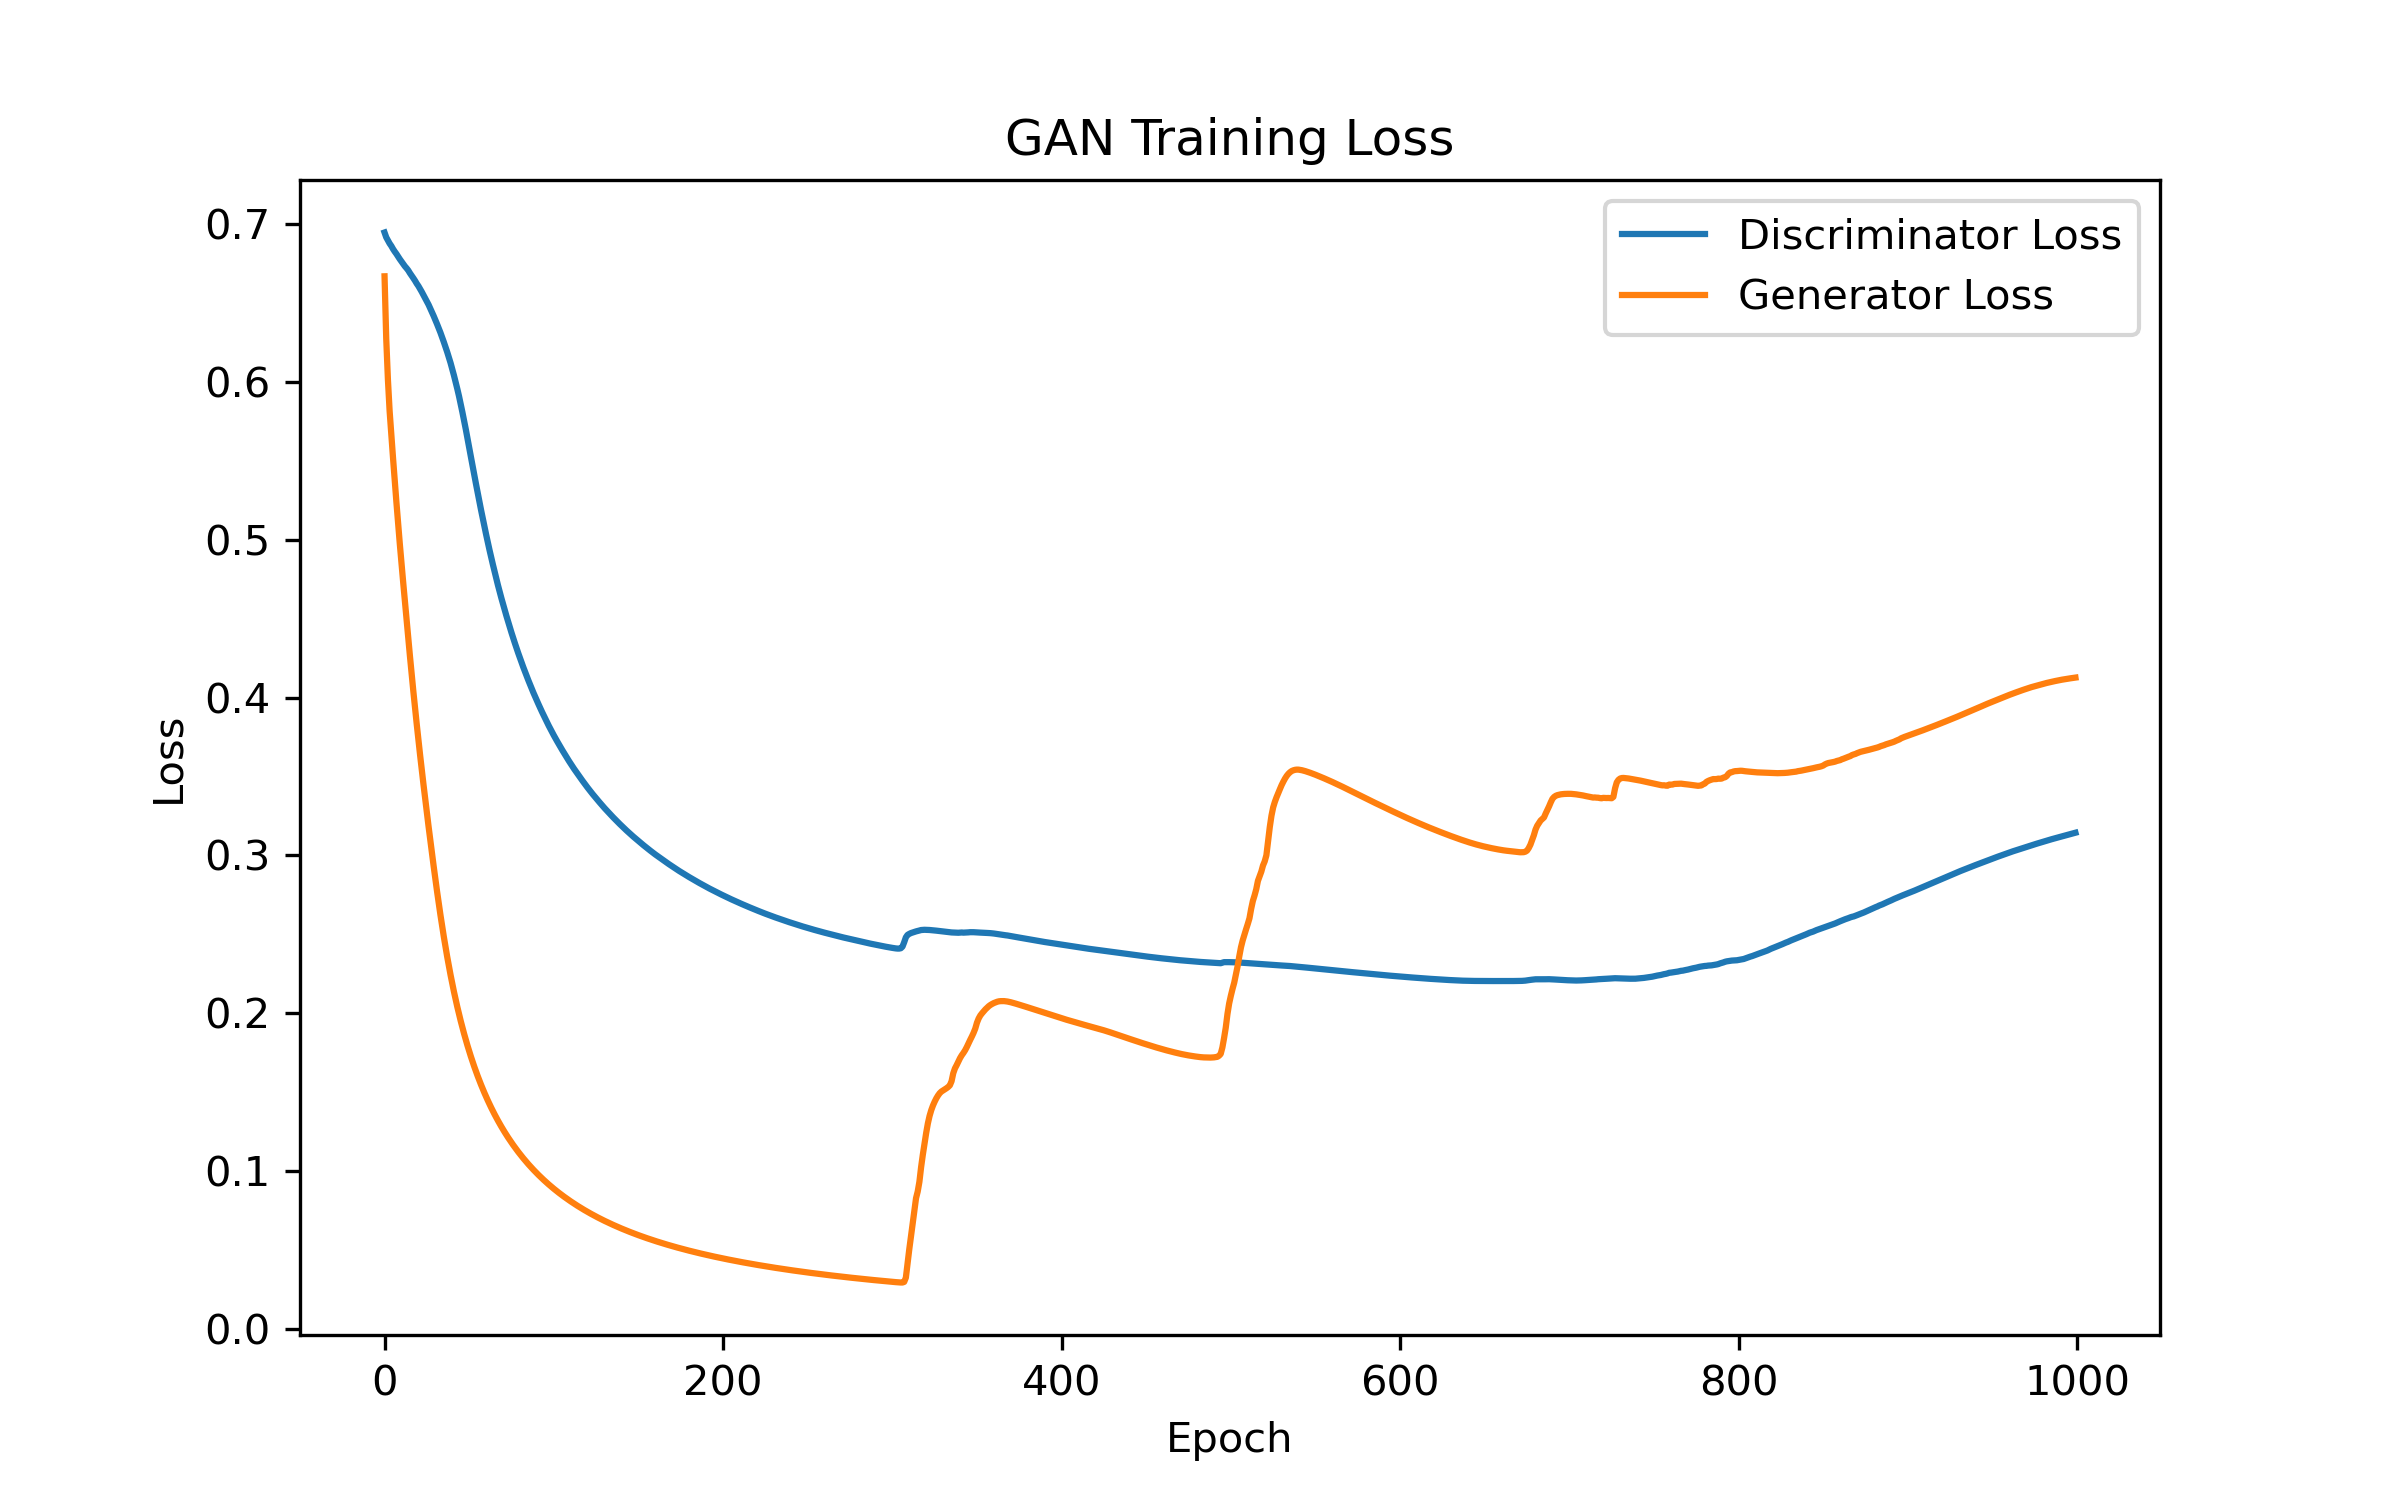
\includegraphics[width=0.9\linewidth]{gan_loss_curve_run_5.png}
\caption{GAN loss curves for Run 5.}
\label{fig:gan_loss5}
\end{figure}

The loss curves demonstrate unstable adversarial behavior during training. Generator and discriminator losses oscillate significantly across runs, which indicates unstable convergence.

% =====================================================
\subsubsection{Discriminator Mistake Analysis}

Figures~\ref{fig:mist1} -- \ref{fig:mist5} show discriminator classification mistakes.

Green labels indicate fake images classified as real.

Red labels indicate real images classified as fake.

\begin{figure}[H]
\centering

\includegraphics[width=\linewidth]{gan_mistakes_run_1.png}
\caption{Discriminator mistakes for GAN Run 1.}
\label{fig:mist1}
\end{figure}

\begin{figure}[H]
\centering

\includegraphics[width=\linewidth]{gan_mistakes_run_2.png}
\caption{Discriminator mistakes for GAN Run 2.}
\label{fig:mist2}
\end{figure}

\begin{figure}[H]
\centering
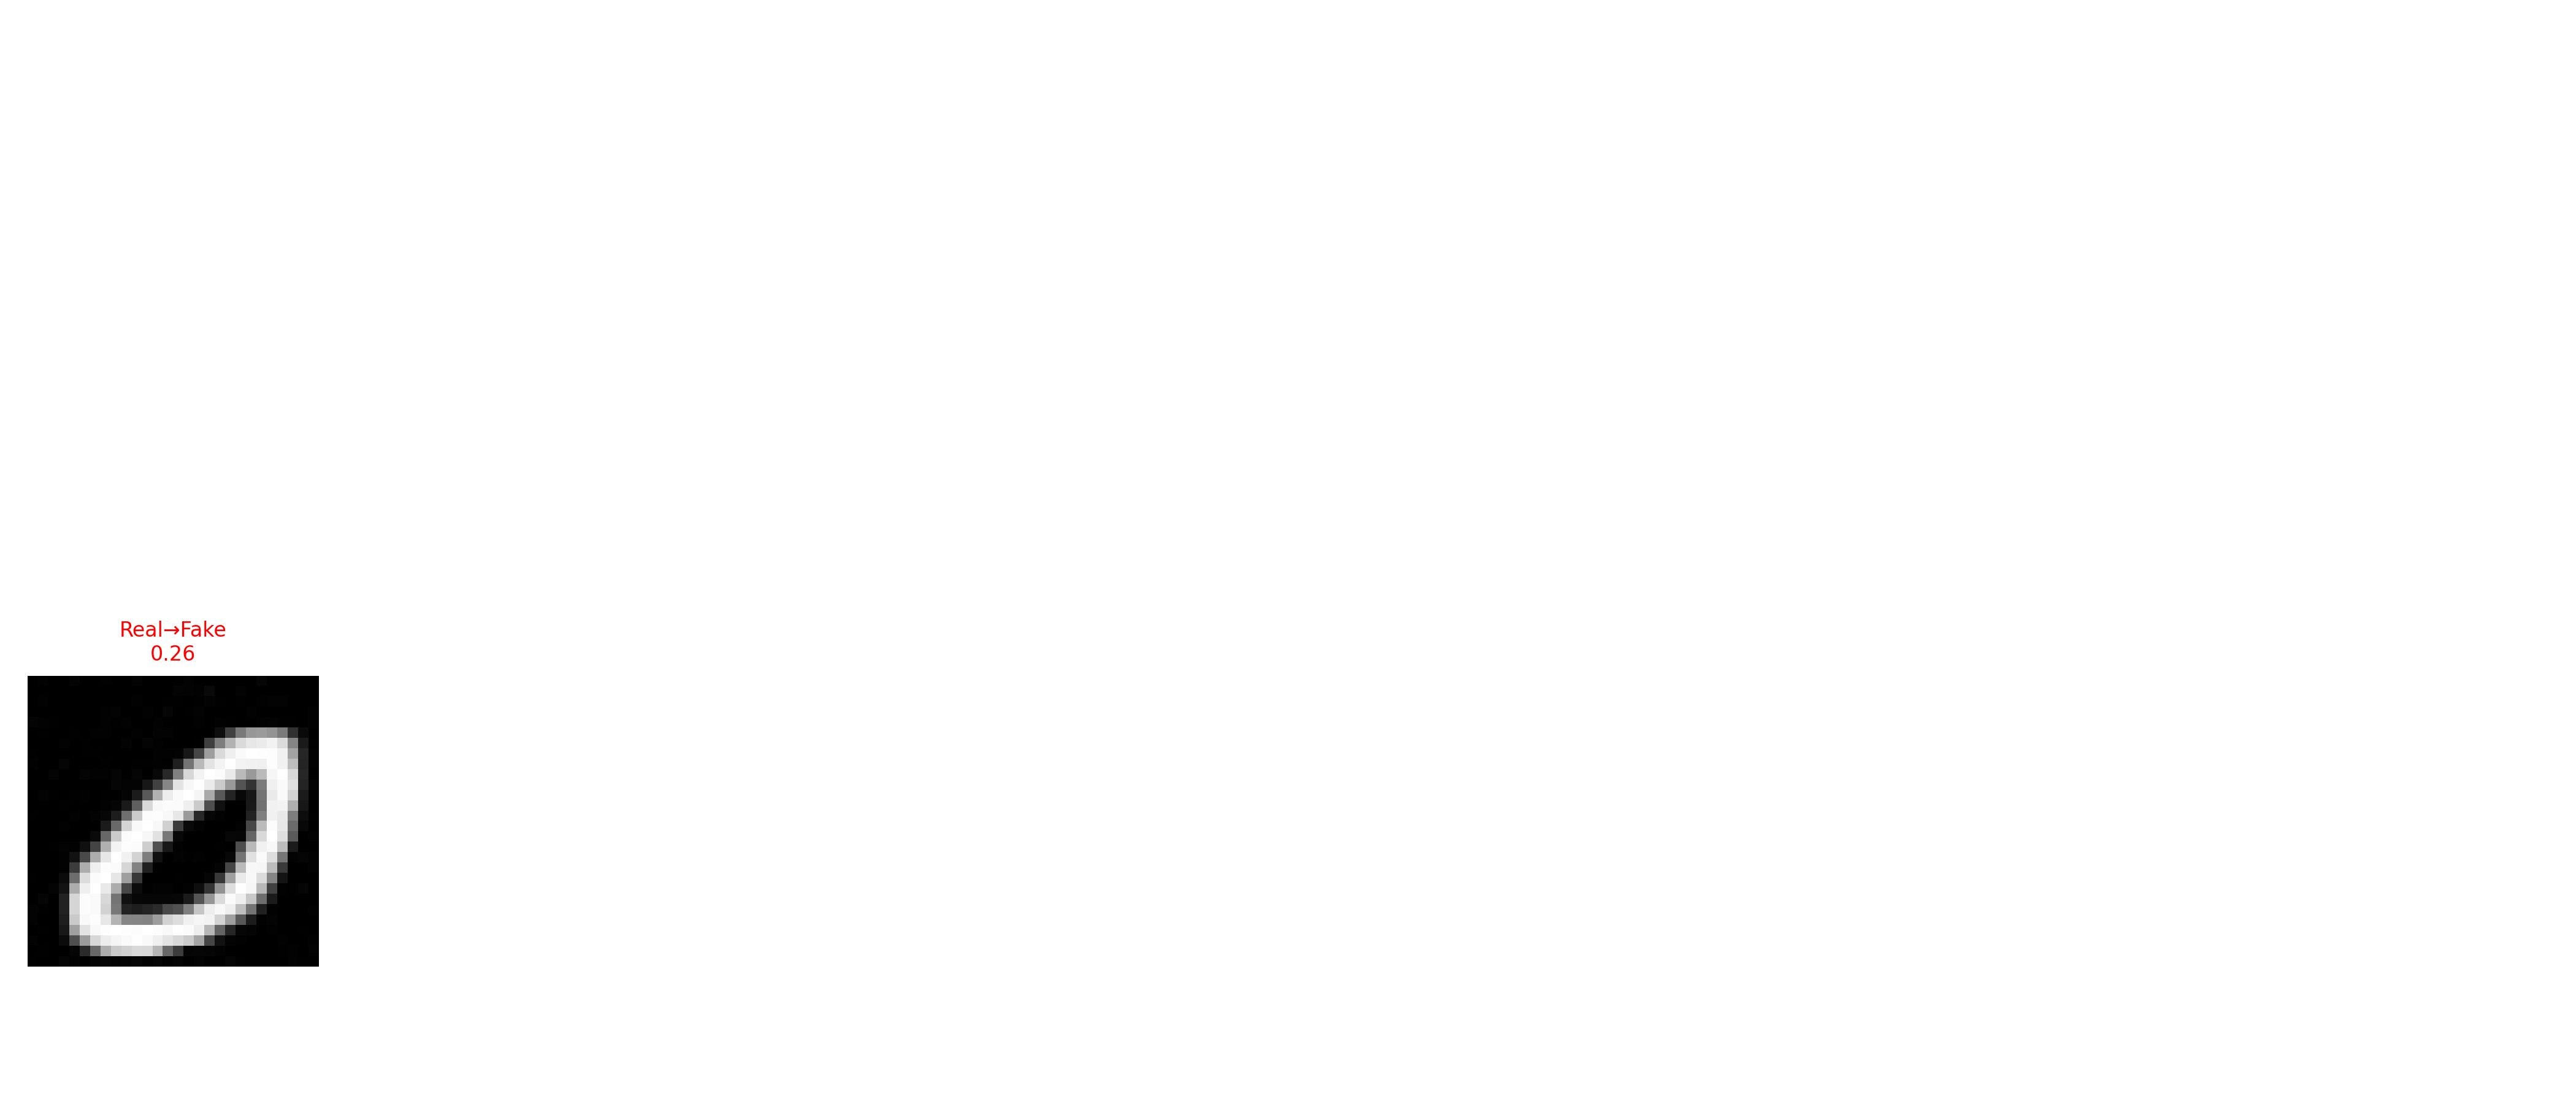
\includegraphics[width=\linewidth]{gan_mistakes_run_3.png}
\caption{Discriminator mistakes for GAN Run 3.}
\label{fig:mist3}
\end{figure}

\begin{figure}[H]
\centering
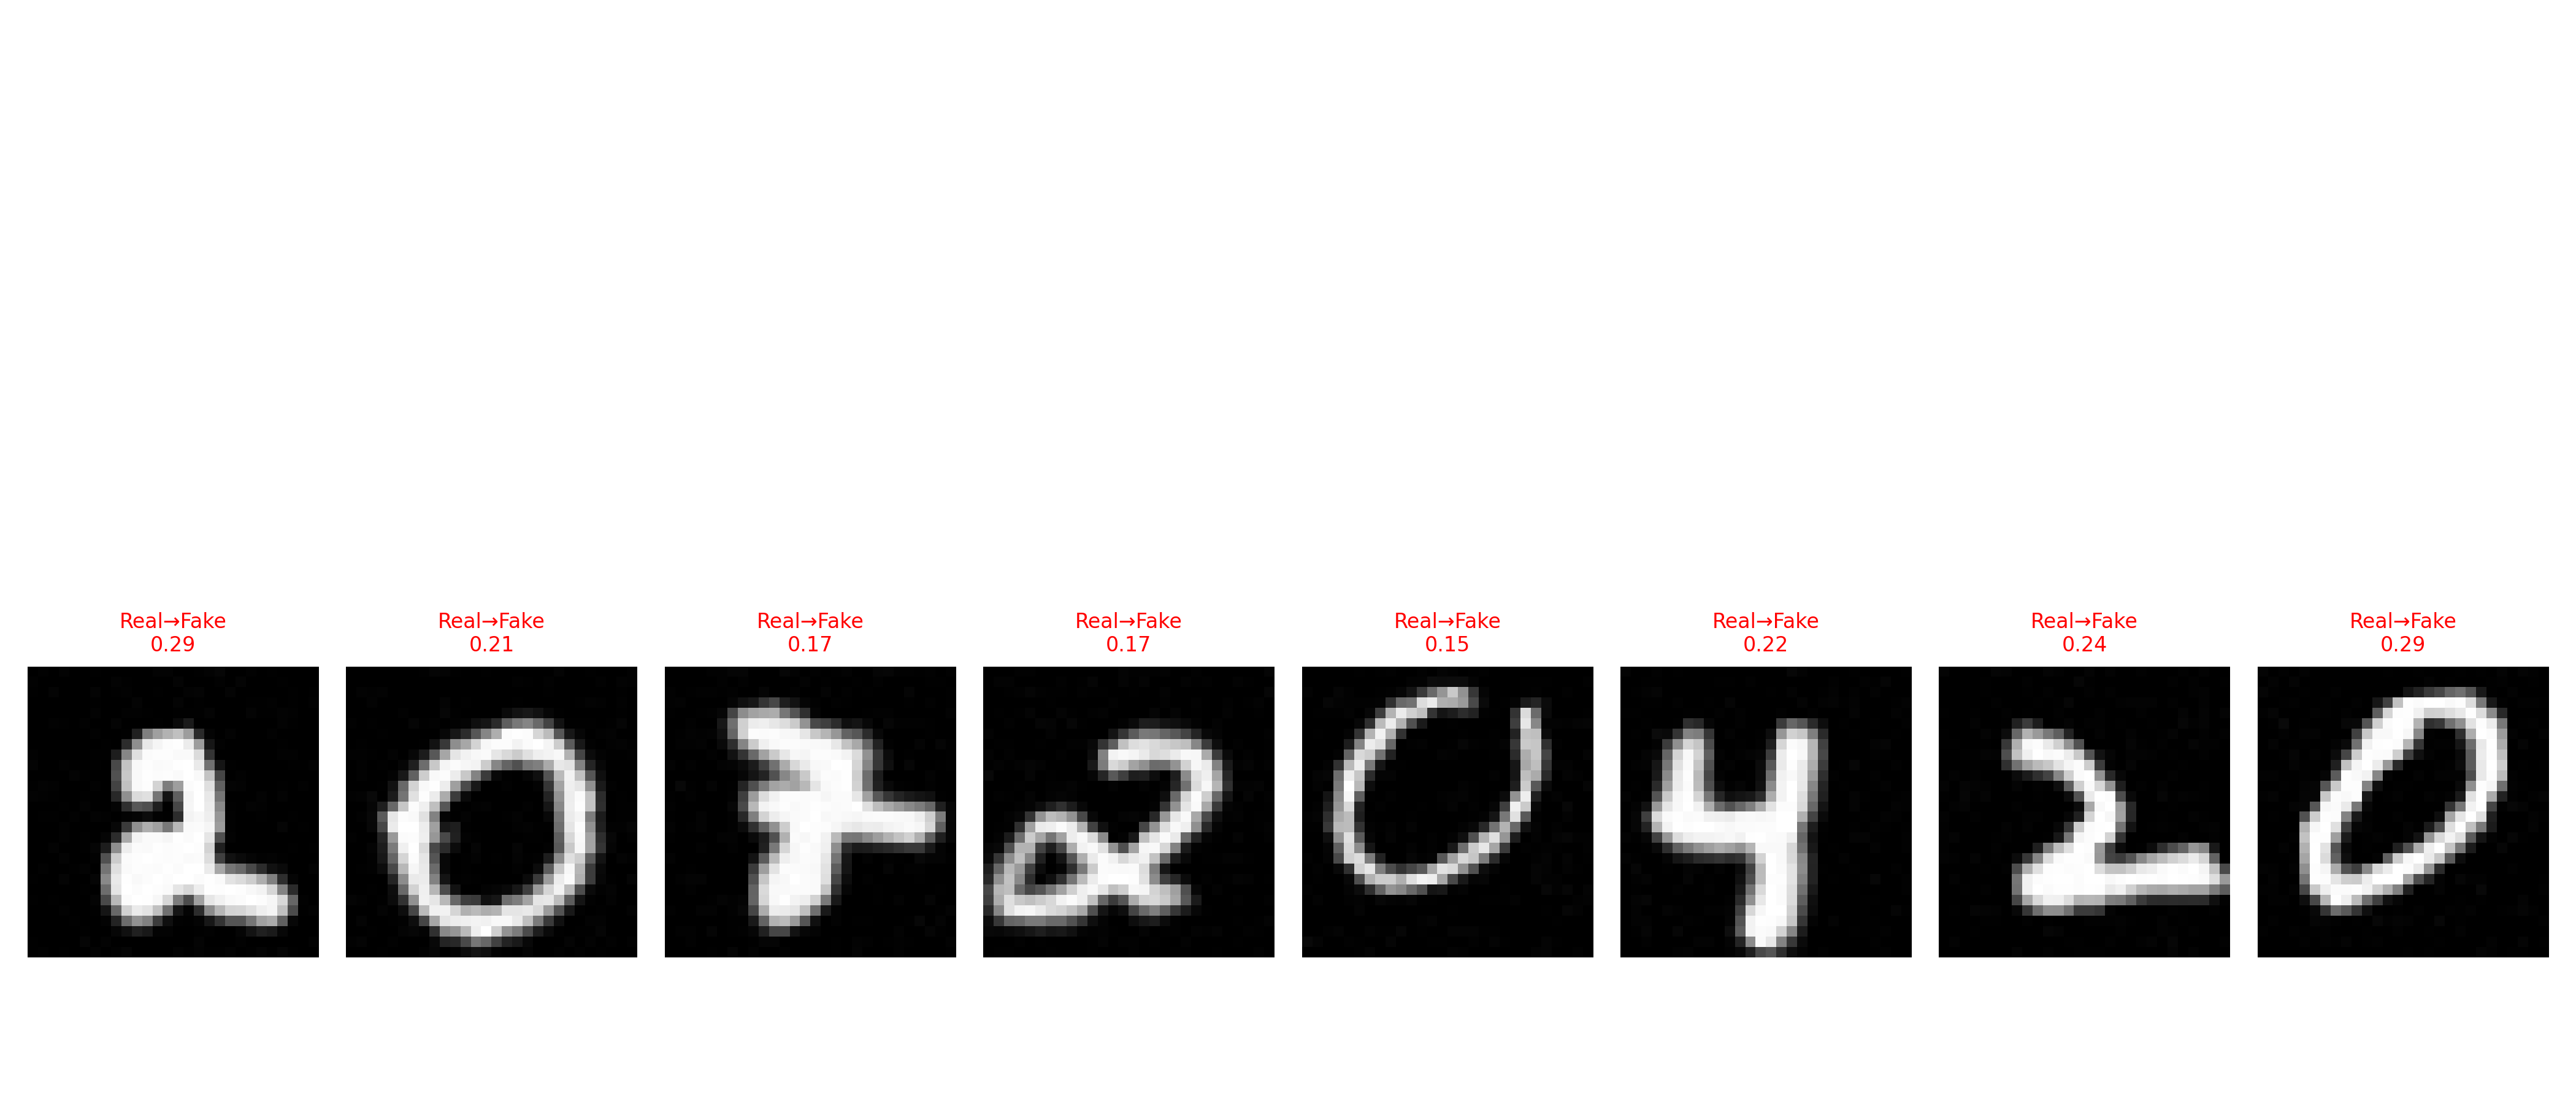
\includegraphics[width=\linewidth]{gan_mistakes_run_4.png}
\caption{Discriminator mistakes for GAN Run 4.}
\label{fig:mist4}
\end{figure}

\begin{figure}[H]
\centering
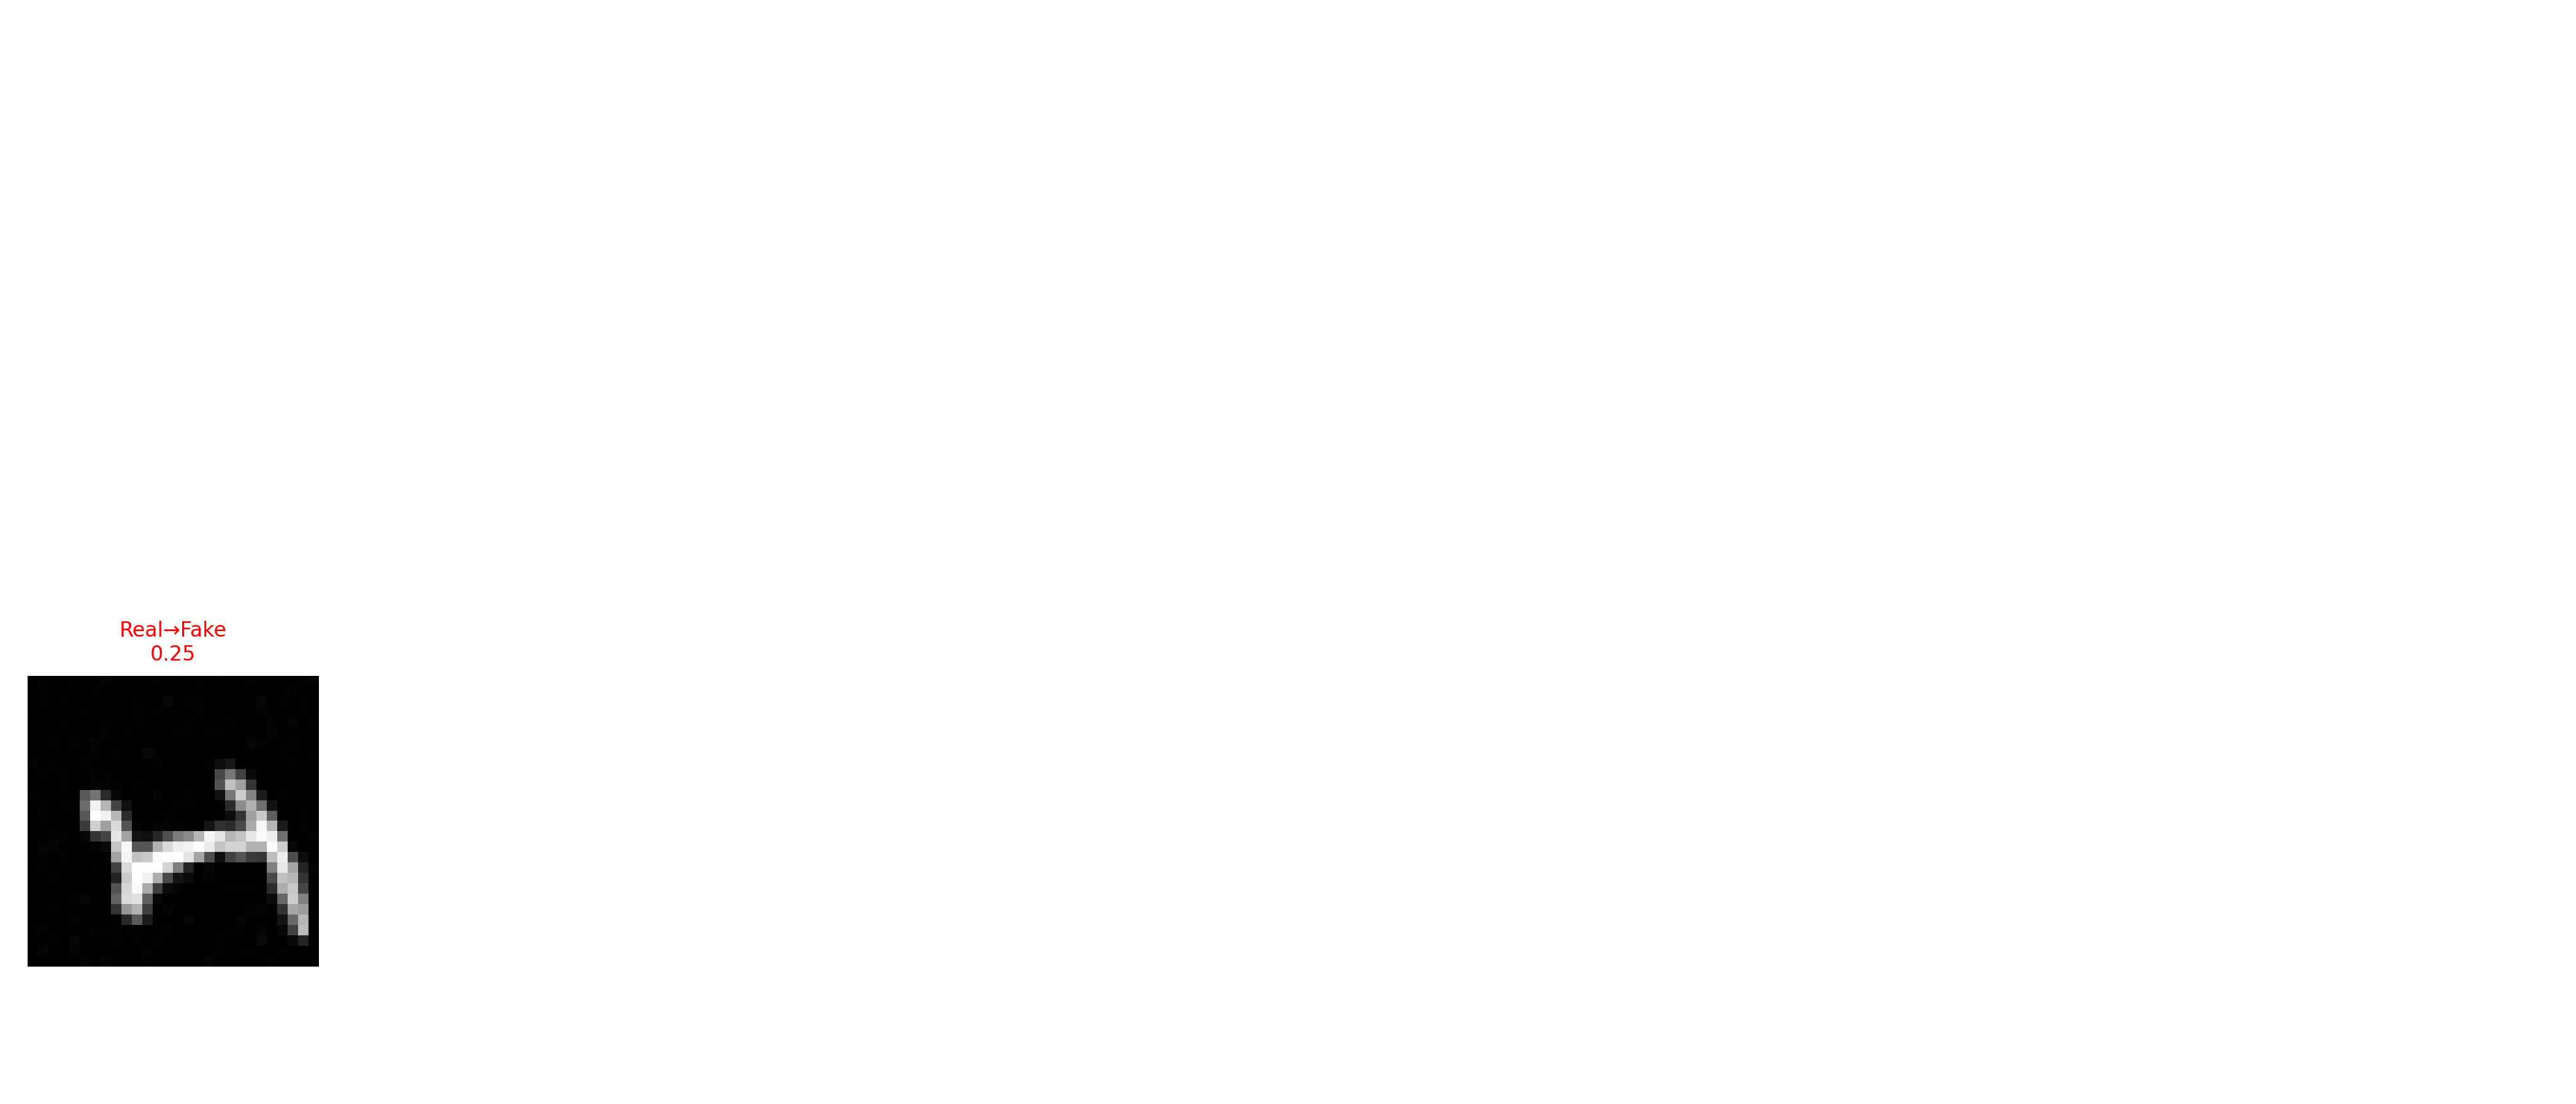
\includegraphics[width=\linewidth]{gan_mistakes_run_5.png}
\caption{Discriminator mistakes for GAN Run 5.}
\label{fig:mist5}
\end{figure}

The discriminator mistakes show that some generated samples successfully fooled the discriminator despite containing visible distortions and unrealistic structures.

% =====================================================
\subsubsection{Generated GAN Samples}

Figure~\ref{fig:ganrun} shows generated samples from one GAN run.

\begin{figure}[H]
\centering
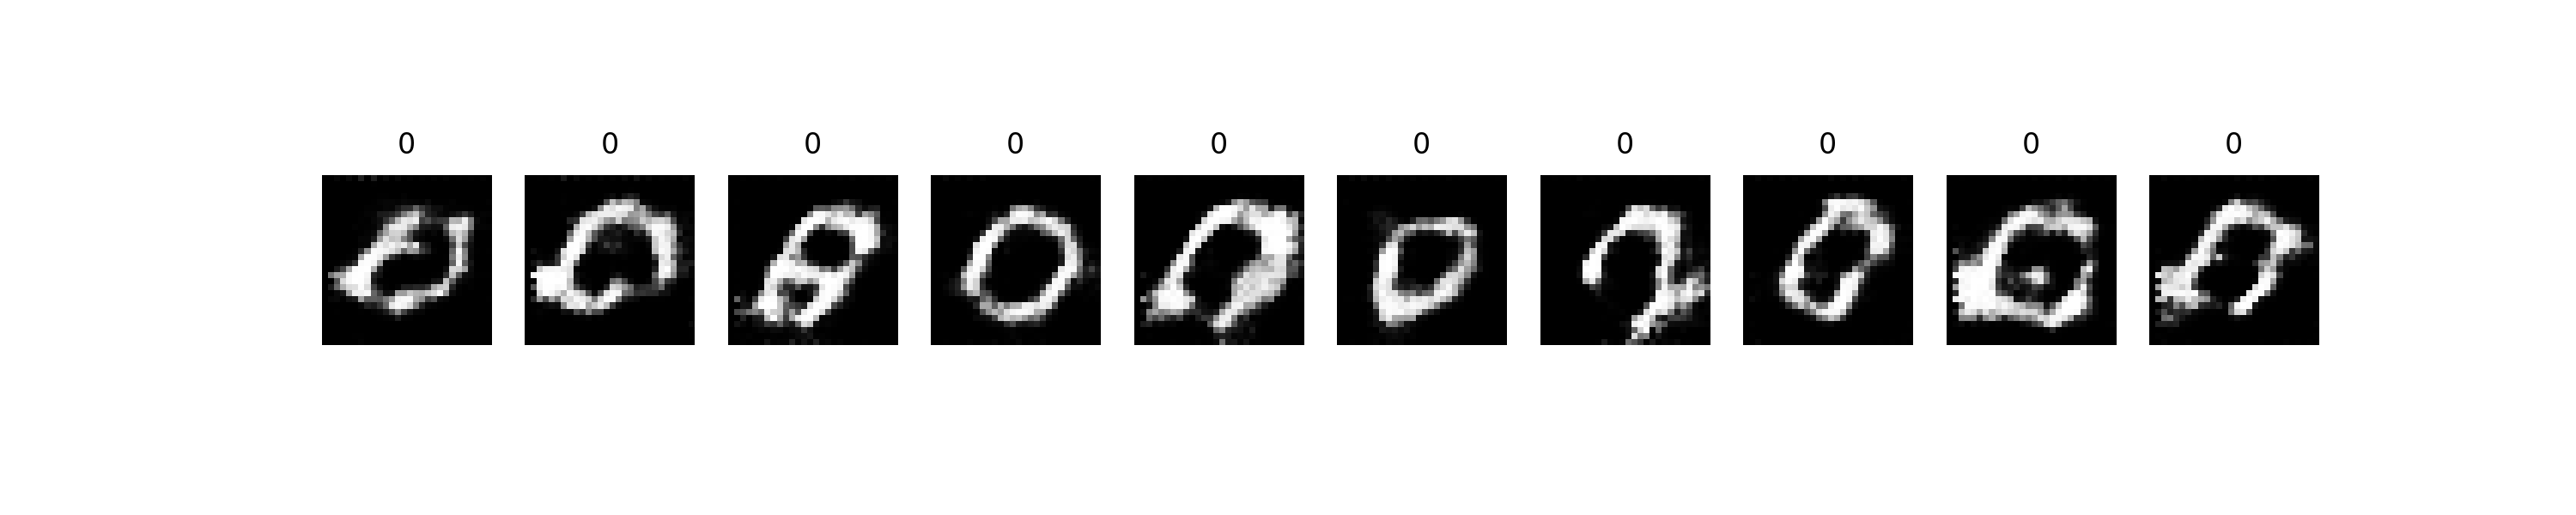
\includegraphics[width=\linewidth]{gan_run_1.png}
\caption{Generated samples from GAN Run 1.}
\label{fig:ganrun}
\end{figure}

The generated digits demonstrate that the GAN learned general digit structure. However, many samples remain blurry or contain artifacts.

Some generated samples appear realistic, while others collapse into noisy or distorted patterns.

% =====================================================
\subsubsection{Synthetic Dataset Construction}

Generated samples were filtered using LeNet-5 classifier confidence.

Three datasets were constructed:

\begin{itemize}
    \item \textbf{Set A}: all generated samples
    \item \textbf{Set B}: confidence $\geq 0.9$
    \item \textbf{Set C}: $0.6 \leq \text{confidence} < 0.9$
\end{itemize}

% =====================================================
\subsubsection{Set A Samples}

\begin{figure}[H]
\centering
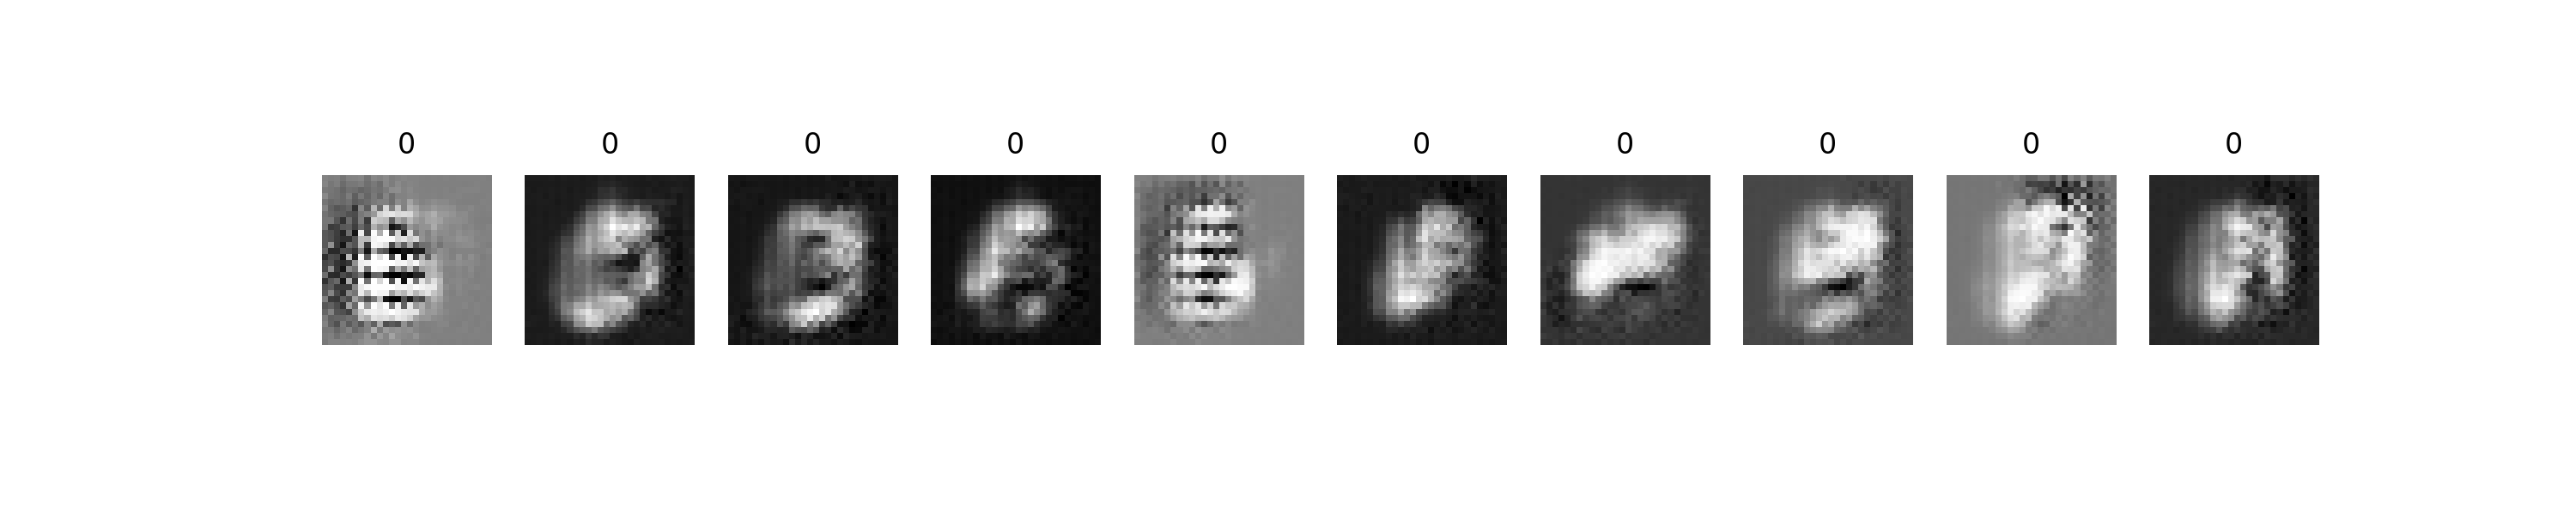
\includegraphics[width=\linewidth]{gan_setA.png}
\caption{Samples from Set A (all generated samples).}
\label{fig:gan_setA}
\end{figure}

Set A includes all generated images. Many samples contain severe artifacts and unstable structures.

% =====================================================
\subsubsection{Set B Samples}

\begin{figure}[H]
\centering
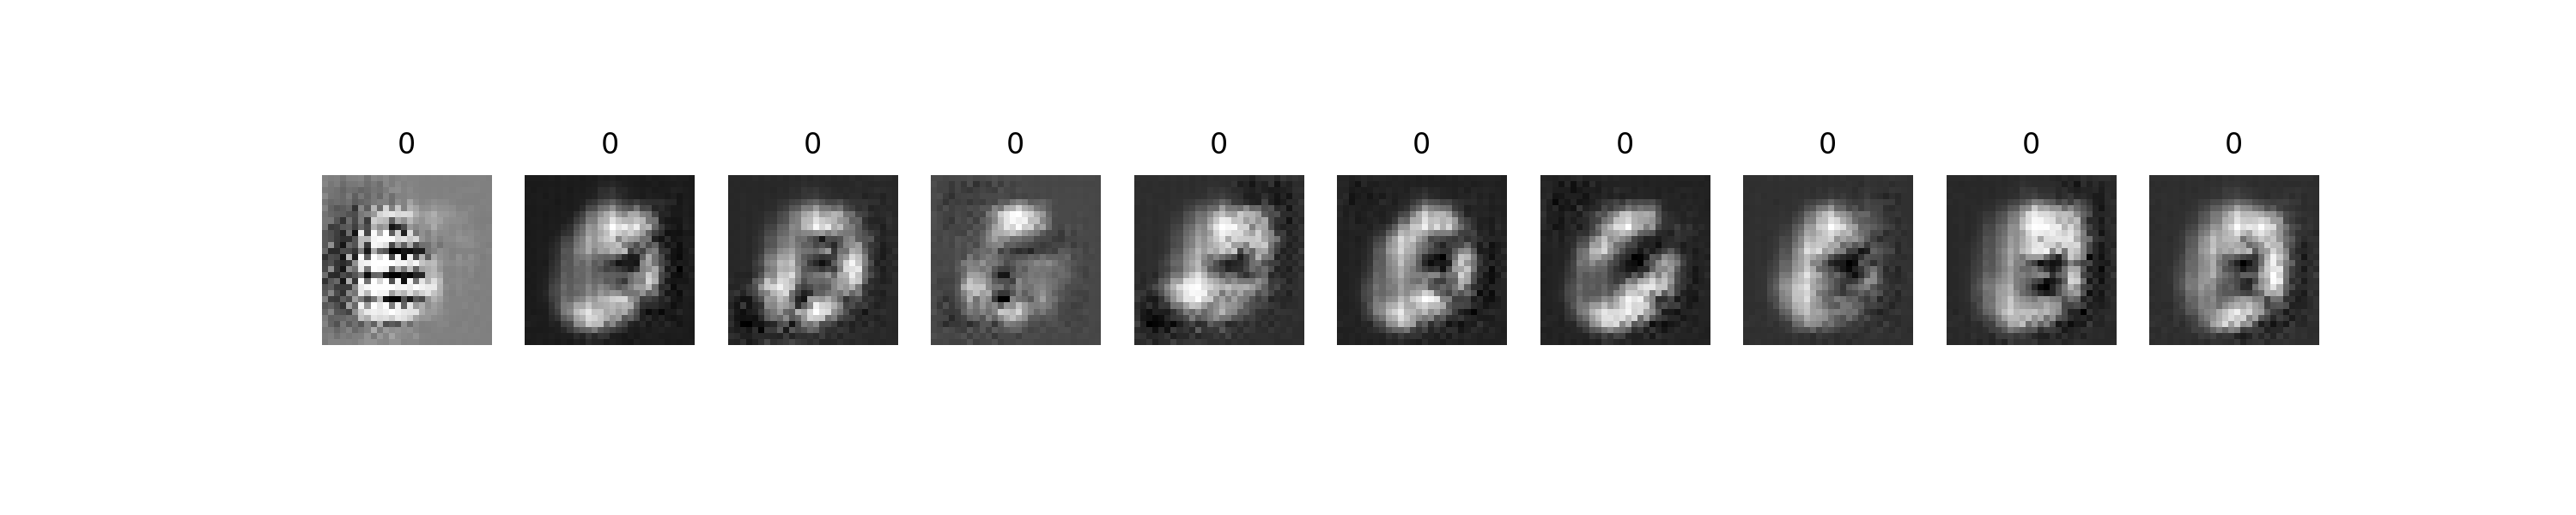
\includegraphics[width=\linewidth]{gan_setB.png}
\caption{Samples from Set B (high-confidence samples).}
\label{fig:gan_setB}
\end{figure}

Set B contains higher-quality samples selected using confidence filtering.

% =====================================================
\subsubsection{Set C Samples}

\begin{figure}[H]
\centering
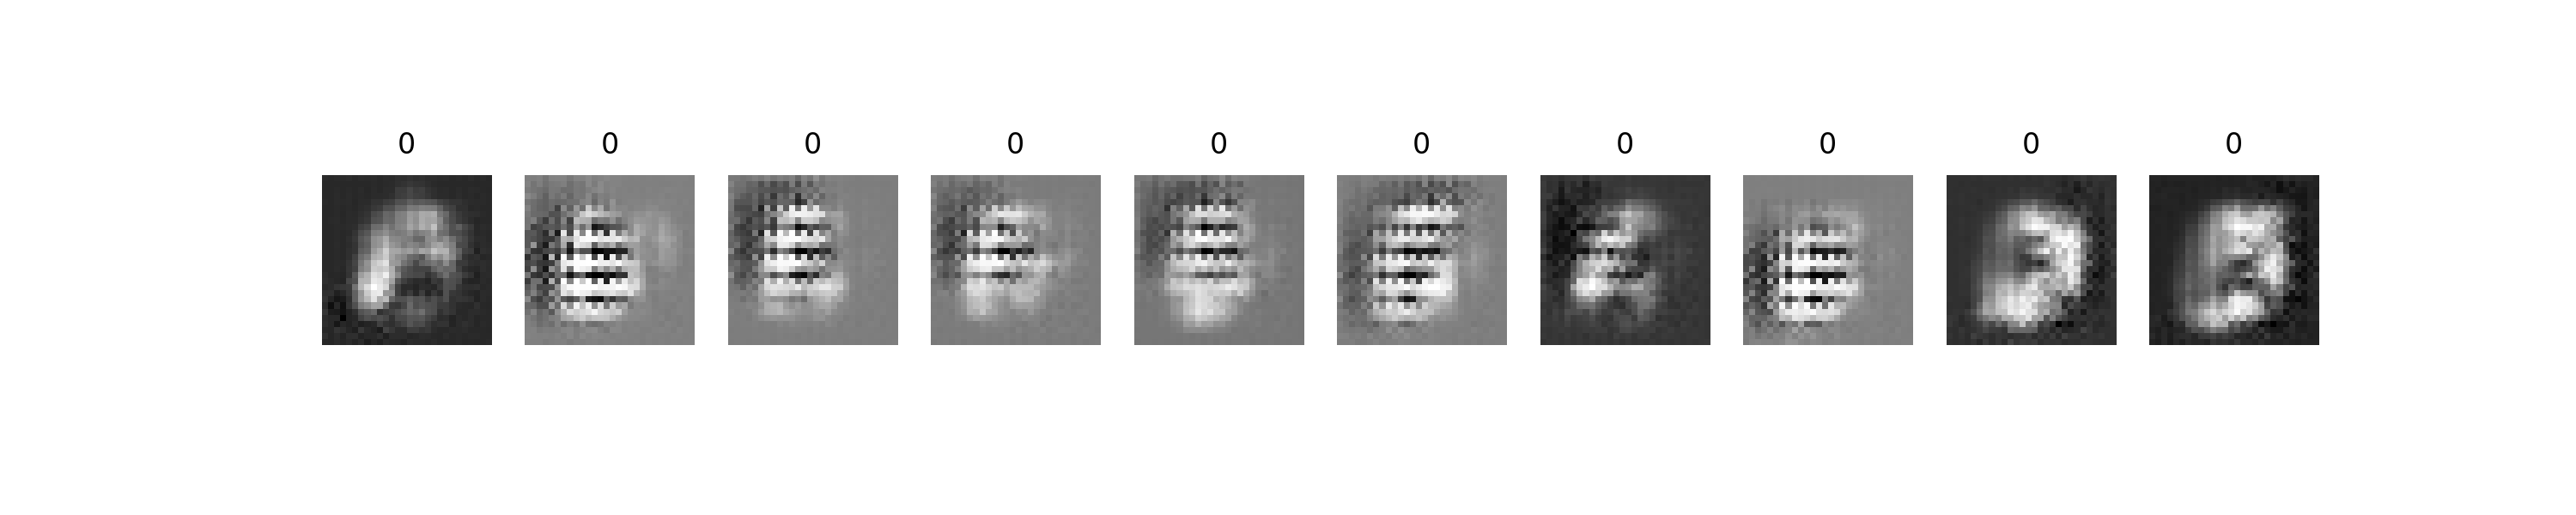
\includegraphics[width=\linewidth]{gan_setC.png}
\caption{Samples from Set C (mid-confidence samples).}
\label{fig:gan_setC}
\end{figure}

Set C preserves moderately confident samples while removing highly corrupted outputs.

% =====================================================
\subsubsection{Experimental Results}

Figure~\ref{fig:gan_results} summarizes classifier performance using GAN-generated synthetic datasets.

\begin{figure}[H]
\centering
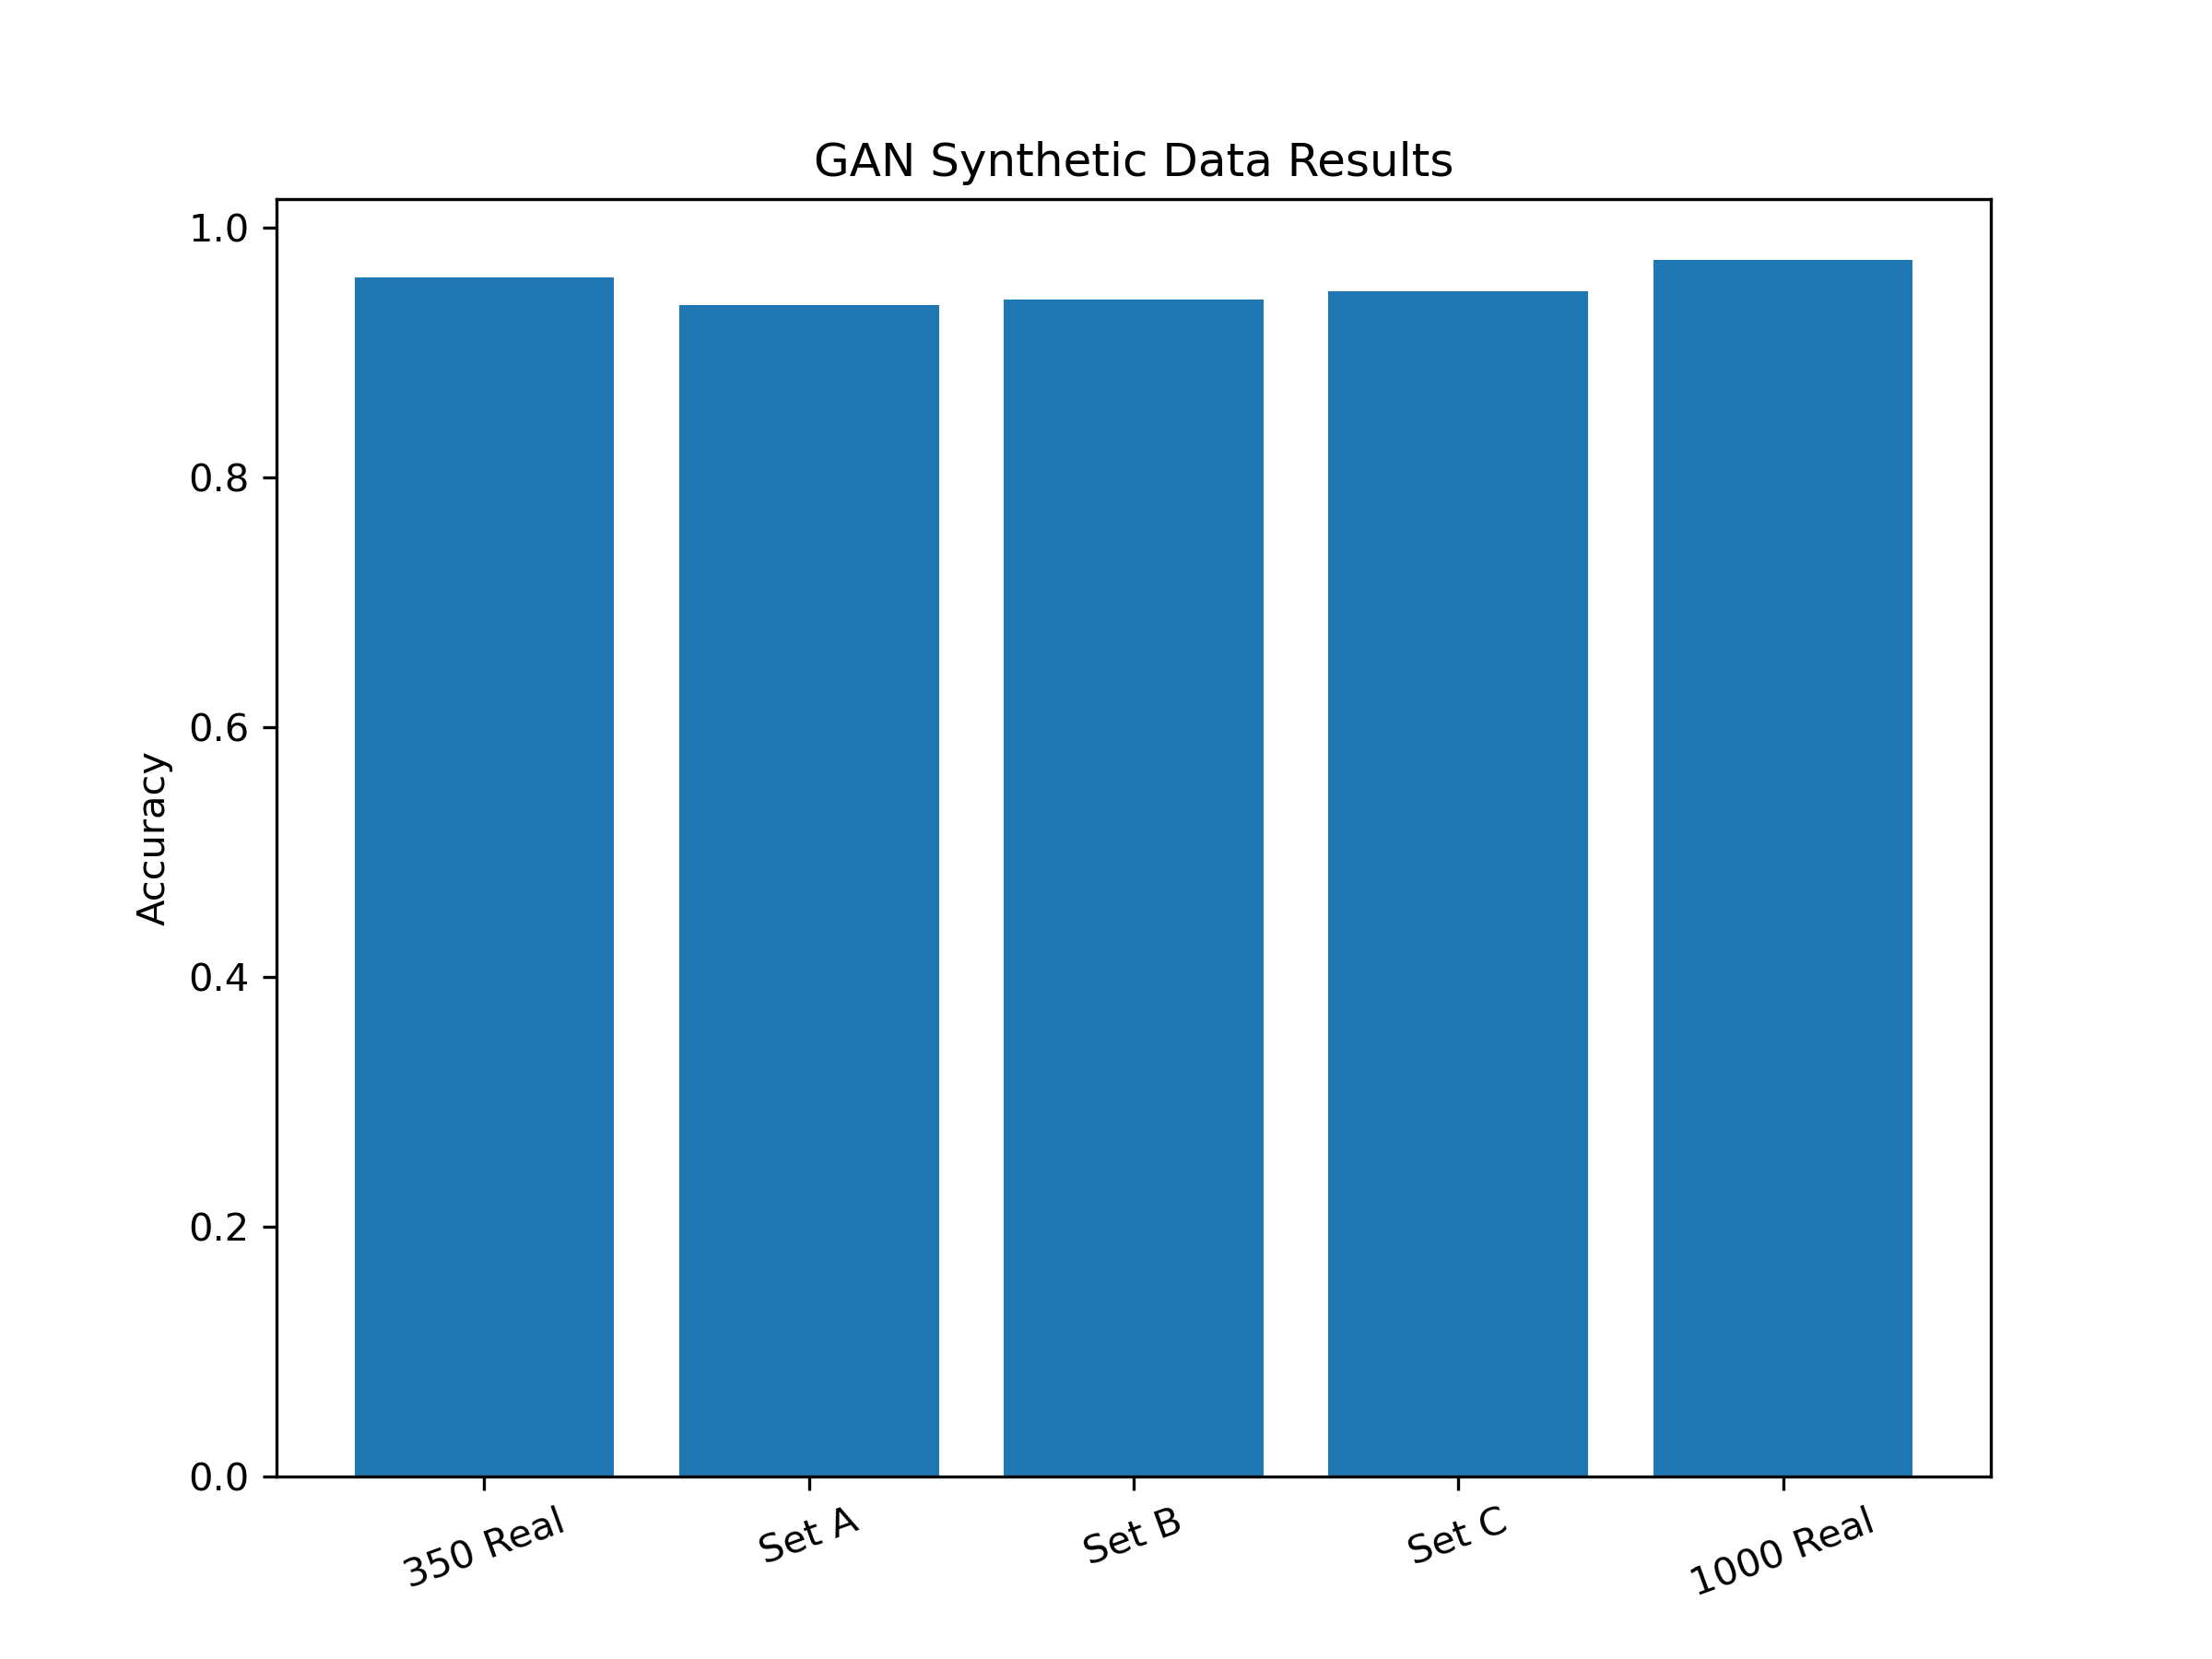
\includegraphics[width=0.8\linewidth]{GAN_results_plot.png}
\caption{Classifier accuracy comparison using GAN-generated datasets.}
\label{fig:gan_results}
\end{figure}

% =====================================================
\subsubsection{Summary Table for Problem 1 and Problem 2}

Table~\ref{tab:final_compare} summarizes the results of both VAE and GAN approaches.

\begin{table}[H]
\centering
\caption{Comparison of VAE and GAN synthetic data strategies.}
\label{tab:final_compare}

\begin{tabular}{|c|c|c|c|}
\hline
\textbf{Model Used} &
\textbf{No. of Examples} &
\textbf{Confidence Level} &
\textbf{Accuracy} \\
\hline

VAE & All generated data & Set A & 93.31\% \\
\hline

VAE & CL $>$ 0.9 & Set B & 95.25\% \\
\hline

VAE & 0.6 $<$ CL $<$ 0.9 & Set C & 95.29\% \\
\hline

GAN & All generated data & Set A & 93.8\% \\
\hline

GAN & CL $>$ 0.9 & Set B & 94.4\% \\
\hline

GAN & 0.6 $<$ CL $<$ 0.9 & Set C & 94.8\% \\
\hline

350 Real Baseline & Real only & --- & 96.36\% \\
\hline

1000 Real Baseline & Real only & --- & 98.17\% \\
\hline

\end{tabular}

\end{table}

% =====================================================
\subsubsection{Discussion}

The experimental results demonstrate several important observations:

\begin{itemize}

\item GAN training was significantly more unstable than VAE training.

\item The adversarial nature of GAN optimization caused oscillations between generator and discriminator performance.

\item Generated GAN samples varied greatly in quality across runs.

\item Some generated digits appeared realistic, while others were blurry or highly distorted.

\item Confidence filtering improved the usefulness of generated samples by removing low-quality outputs.

\item Set B and Set C consistently performed better than Set A because filtering removed unrealistic samples.

\item Despite improvements, GAN-generated data still did not outperform the real-only baseline.

\item Compared to Assignment 2 augmentation, traditional augmentation remained more stable and reliable.

\item The experiments show that synthetic data can partially compensate for limited datasets, but fully replacing real data remains difficult.

\end{itemize}

% =====================================================
\subsubsection{Conclusion}

A Conditional GAN was successfully implemented for MNIST handwritten digit generation using a highly limited dataset.

The generated samples demonstrated that the GAN learned meaningful digit structures; however, training instability caused large quality variations across runs.

Visual inspection confirmed that some generated samples were realistic while others suffered from mode collapse, blur, and severe artifacts.

Experimental evaluation showed that confidence-based filtering improved classifier performance by selecting more reliable synthetic samples.

Overall, GAN-generated data partially reduced the need for real data, but the results indicate that synthetic GAN samples still cannot fully replace real training samples.

Compared to VAE generation and traditional augmentation, GAN training was less stable and more sensitive to initialization and adversarial dynamics.

\endgroup